\documentclass[ oneside,% the name of the author
                    author={Cassie Qing Tang},
                % the degree programme: BSc, MEng, MSci or MSc.
                    degree={BSc},
                % the dissertation    title (which cannot be blank)
                     title={An Automated Response System for Disrupting Online Pet Scamming \\ },
                % the dissertation subtitle (which can    be blank)
                    subtitle={ }]{dissertation}

\usepackage[english]{babel}
\usepackage[nottoc]{tocbibind}
\usepackage{graphicx}
\usepackage{subcaption}
\usepackage{float}
\usepackage[list=true]{subcaption}
\usepackage{caption}
\usepackage[utf8]{inputenc}
\usepackage{hyperref}
\usepackage{listings}
\usepackage{fancyvrb}
\usepackage[a4paper, margin=1in]{geometry}
\usepackage{booktabs}
\usepackage{graphicx}
\usepackage{array}
\usepackage{hyperref}
\usepackage{textcomp}

\begin{document}

\maketitle
% \fronmatter

\chapter*{Abstract}
In response to the increasingly serious threat of online pet scams, this project has successfully developed an automated response system. This system manages the entire scam defence process, from obtaining scam links to automatic form filling, and then to email interaction with scammers. In a 31-day experiment, the system successfully consumed the time and resources of scammers, effectively disrupting with pet scam activities. Based on four common consumer personalities, I designed the email response strategies used in the experiment, namely Investigator, Newbie, Bargainer, and Impatient Consumer. The results indicate that the response using the Newbie strategy can most effectively extend the interaction time with more scammers, thereby significantly interfering with scam activities, which is also consistent with my research hypothesis. This project not only helps the public to deeply understand and defend online pet scams, but also provides strategies for combating such scams. It offers valuable insights for fraud defence technologies in the field of cybersecurity.
\\

The points below outline the tasks completed and the time invested in this research:

\begin{itemize}
  \item I spent a total of 40 hours reading literature related to pet scams, designing the system architecture, and formulating experimental procedures.
  \item I spent approximately 90 hours building the system, during which I wrote 1,620 lines of Python source code. This mainly included five main scripts that carry out scam defence processes, as well as two programs that set different reply strategies and interact with the GPT language model.
  \item I spent 10 hours testing the entire system.
  \item I spent 10 hours organising the data obtained from the experiment and completed the statistical analysis of the valid data.
\end{itemize}


\chapter*{Acknowledgements}
I would like to express my special thanks to my supervisor, Dr Matthew Edwards, for his help and guidance in this project.
\\
\\
I would also like to give my thanks to School of Engineering for inviting me into UoB Computer Science OpenAI Team, which reimburses me the cost of using the different APIs of \href{https://openai.com/}{OpenAI}.
\\
\\
Sign up for GitHub Student Developer Pack provides me free access to many useful tools, involving \href{https://www.mailgun.com}{Mailgun} and \href{https://www.name.com}{Name.com}. Appreciate the resources it provides!

\makedecl


\tableofcontents
\listoffigures
\listoftables

\chapter*{Ethics Statement}
An ethics application for this project was reviewed and approved by the faculty research ethics committee as application 17599.


\chapter*{Supporting Technologies}
I created my system based on an open-source GitHub repository from \url{https://github.com/an19352/scambaiter_back}. By extending and altering its code to fit my needs.
\\
\\
I integrated two GPT models, specifically \texttt{GPT-3.5-turbo-0125} and \texttt{GPT-4-0125-preview}, into my system via their APIs to ensure the functionality of an automatic email reply feature. One necessary API key was acquired and configured using the resources available at \url{https://openai.com/}.
\\
\\
I applied my own domain name from \url{https://www.name.com/} in order to generate a large number of bait-email addresses.
\\
\\
I obtained a mailgun API key and build a mailbox server on \url{https://www.mailgun.com/}, which can support emails receiving, sending and tracking.

\chapter*{Notation and Acronyms}
\begin{quote}
\noindent
\begin{tabular}{lcl}
AFF                 &:     & Advance Fee Fraud    
 \\ 
HTTP/HTTPS          &:     & Hypertext Transfer Protocol/Hypertext Transfer Protocol Secure
 \\ 
HTML                &:     & Hypertext Markup Language
\\
XML                 &:     & Extensible Markup Language
\\
Regex               &:     & Regular Expression
\\
NLP                 &:     & Natural Language Processing
\\
SSL                 &:     & Secure Sockets Layer
\\
JSON                &:     & JavaScript Object Notation
\\
A*                  &:     & A-star
\\
GPT                 &:     & Generative Pre-Trained Transformer
\\
API/APIs            &:     & Application Programming Interface
\\
URL/url             &:     & Uniform Resource Locator
\\
UNIX/UNICS          &:     & UNiplexed Information Computing System
\\
DNS                 &:     & Domain Name System
\\
CSS                 &:     & Cascading Style Sheets
\\
DOM                 &:     & Document Object Model
\\
TPM                 &:     & Tokens Per Minute

\end{tabular}
\end{quote}


\mainmatter

\chapter{Introduction}
\label{chap:context}
In the definition of online scam, both advance fee and non-delivery frauds can be defined as a social engineering attack. The former is that fraudsters often promise their victims goods or more money in order to convince them to pay a fee upfront \cite{claude_toward_2014}. This scheme has been widely applied to lottery scams, inheritance scams, romance scams, etc. While the latter can be seen as a concrete realisation of the former that victims could never receive the goods even though they have sent the payment \cite{whittaker_understanding_2020}. In recent years, the happen of these two types of fraud have become increasingly frequently with the growing demand for online shopping and the development of logistics. According to the Internet Crime Report for 2019 \cite{noauthor_2019_nodate}, more than 60,000 Americans experienced non-delivery scams during the year, and another 14,607 Americans reported that they had been subjected to the AFF. The total amount of money involved in both reached nearly \$300 million. The newly released annual report for 2023 shows this amount has risen to \$450 million, even as the complaint count for the corresponding type of fraud has decreased \cite{noauthor_2023_nodate}. Simultaneously, the UK is also witnessing a similar rise in the prevalence of AFF with a substantial 549\% increase noted in March 2023 compared to three years prior \cite{stripe_crime_2023}. 
\\

Pet fraud is a typical scam involving AFF and non-delivery frauds. Scammers usually register a domain name at a very low cost to create their own e-commerce website. They attract consumers to purchase non-existent pets by placing a large number of online advertisements on social media such as Facebook and offering low prices \cite{price_resource_2020}. In order to quickly gain the trust of potential victims, scammers build seemingly legitimate websites. They prominently display on the homepage that they have joined some credible real organisations, or claim to be certified as top sellers of certain dog breeds, and display some fake consumer purchase reviews and services they have provided \cite{price_resource_2020}. In addition, most of the cute pet photos displayed on scam websites are sourced from other legitimate platforms \cite{better_business_bureau_bbb_2017}. Scammers attach the name, breed, age, and even fabricated stories about the pet alongside these stolen photos. People interested in owning pets are more likely to desire a purchase after seeing this information. They typically reach out to the scammers via the WhatsApp number, email address, or other contact details provided on the webpage. Alternatively, they may actively complete the contact form on the webpage.
\\

At this stage, most victims are almost trapped in pet scams. Scammers guide them towards private communication channels that are not supervised by regular e-commerce platforms, using pre-written scam templates to make false promises \cite{ipata_current_nodate}. Once trust is established, victims are asked to pay for pets using non-refundable payment methods like Western Union or MoneyGram, subsequently receiving a tracking number and a URL for a delivery website to track their orders \cite{price_resource_2020}. Unexpectedly, these websites are also controlled by the scammers. These `pet orders' soon encounter various fictitious transportation and medical issues, resulting in continuous delays in the transaction \cite{price_resource_2020}. Capitalising on the victims' emotional investment, the scammers continuously request additional fees with new excuses until the victims realise they have been deceived. Consequently, the victims not only fail to receive the pets but also lose a significant amount of money. A report indicates that about two-thirds of scam victims in England and Wales have experienced mental health and sleep issues \cite{shaw_report_2024}, which is confirmed by Kanetria Hutcherson's experience \cite{better_business_bureau_bbb_2017}.
\\

The earlier data comes from a 2015 report by the Federal Trade Commission (FTC) in the United States, which recorded approximately 37,000 pet-related complaints \cite{better_business_bureau_bbb_2017}. The Better Business Bureau's (BBB) recent research indicates that, since 2017, pet scams have represented a quarter of online shopping fraud cases in the US, with the average yearly financial loss for victims continuing to rise \cite{better_business_bureau_bbb_2022}. Similar problems have been reported worldwide in recent years. For instance, Lloyds Bank in the UK noted a significant rise in pet scam complaints according to their released statistics \cite{lloyds_bank_fraudsters_2023}. Relevant research in Australia and Canada also reflects this trend \cite{better_business_bureau_bbb_2017}.
\\

Despite the above reports have revealed the mature modus operandi of pet scam gangs and their increasingly detrimental impact on society, pet scams have not received as much attention as other similar scams, such as romance scams. Current research and countermeasures are primarily focused on helping the public identify and prevent pet scams. This includes the reporting and searching functions provided by \href{https://www.ipata.org/pet-scams}{IPATA} and \href{www.petscams.com}{Petscams}, as well as \href{www.aa419.org}{AA419}, which operates a fake website database. Moreover, there are some technical development projects, such as the development of \textit{Scammed Posts Detector} \cite{norazman_development_2014} and the research of \textit{Automated classification of pet scam websites} \cite{mehmedov_automated_2021}. However, there is still a lack of targeted research that can effectively defend and disrupt such scams.
\\

This article will further investigate the field of pet scams. Based on the current operational mode of pet scams, an automatic response system that disrupts pet scams has been developed. This system is built on the basis of an expandable Scam-baiting Mail Server \cite{an19352_an19352scambaiter_back_2023}, aiming to contribute to the resistance and disruption of pet scams. As part of the project, multiple web crawlers will be built to extract and process various data. This includes the homepage URLs and the contact form pages on pet scam websites, as well as the implementation of automatic form filling. On the other hand, the system also needs the functionality to send and receive emails, as scammers will initiate email contact after receiving the form application. Thus, we conducted a 31-day experimental interaction with pet scammers by constructing our own email server and devising various response strategies, namely Investigator, Newbie, Bargainer, and Impatient Consumer. After the experiment, relevant information and data will be integrated and analysed to determine the most effective response strategy. Finally, the project results are discussed comprehensively in terms of the success rate of script execution and the response rate of emails. The project execution intends to provide the public with powerful anti-pet scam strategies directly. Additionally, the automatic form-filling script can be paired with other advertisement scam detectors, such as the \textit{Scam Detection in Online Classified Advertisements} developed by Hamad Alsaleh \cite{alsaleh_scam_2017}. This can further assist more researchers and anti-fraud organisations in understanding and combating online fraud.
\\

Therefore, the specific objectives of this project can be summarised as the following key points:

\begin{itemize}
  \item Implement the automatic form-filling script and prove its feasibility through experimentation.
  \item Identify the best personality to disrupt pet scams, contributing to a safer online environment.
  \item Increase the understanding of pet scammers and their common methods used in emails, to help myself and others improve awareness of pet scams.
\end{itemize}


\chapter{Technical Background}
\section{Petscams.com}
The data for pet scam websites in this study was sourced from a volunteer organisation called \href{https://www.petscams.com}{Petscams}. This organisation operates a website, using the same domain name, to list fraudulent pet sales and shipping sites \cite{brady_fighting_2024}. \href{https://www.petscams.com}{Petscams.com} is an effective and free platform offering a range of security services to alert the public about the danger of those websites. These services include victim reporting and comment systems, fraudulent website analysis, verification, classification, and continuous article updates. They also provide access of these data to law enforcement agencies to better disrupt and combat scammer activities. Beyond that, they have been a valuable resource for other researchers. For instance, their victim report system significantly contributed to a pet scam case study published in 2020 \cite{whittaker_understanding_2020}.
\\

Figure \ref{fig:pic1} illustrates how articles on this website maintain consistent HTML structural features in the developer mode of the Chrome browser. It's clear to see each article is nested within an $<$article$>$ tag, which is part of the HTML5 semantic markup, used to define independent content modules on the website. Importantly, each article's title, which the suspected fraudulent domain information, is placed within the $<$h2$>$ tag. 
\begin{figure}[H]
\centering
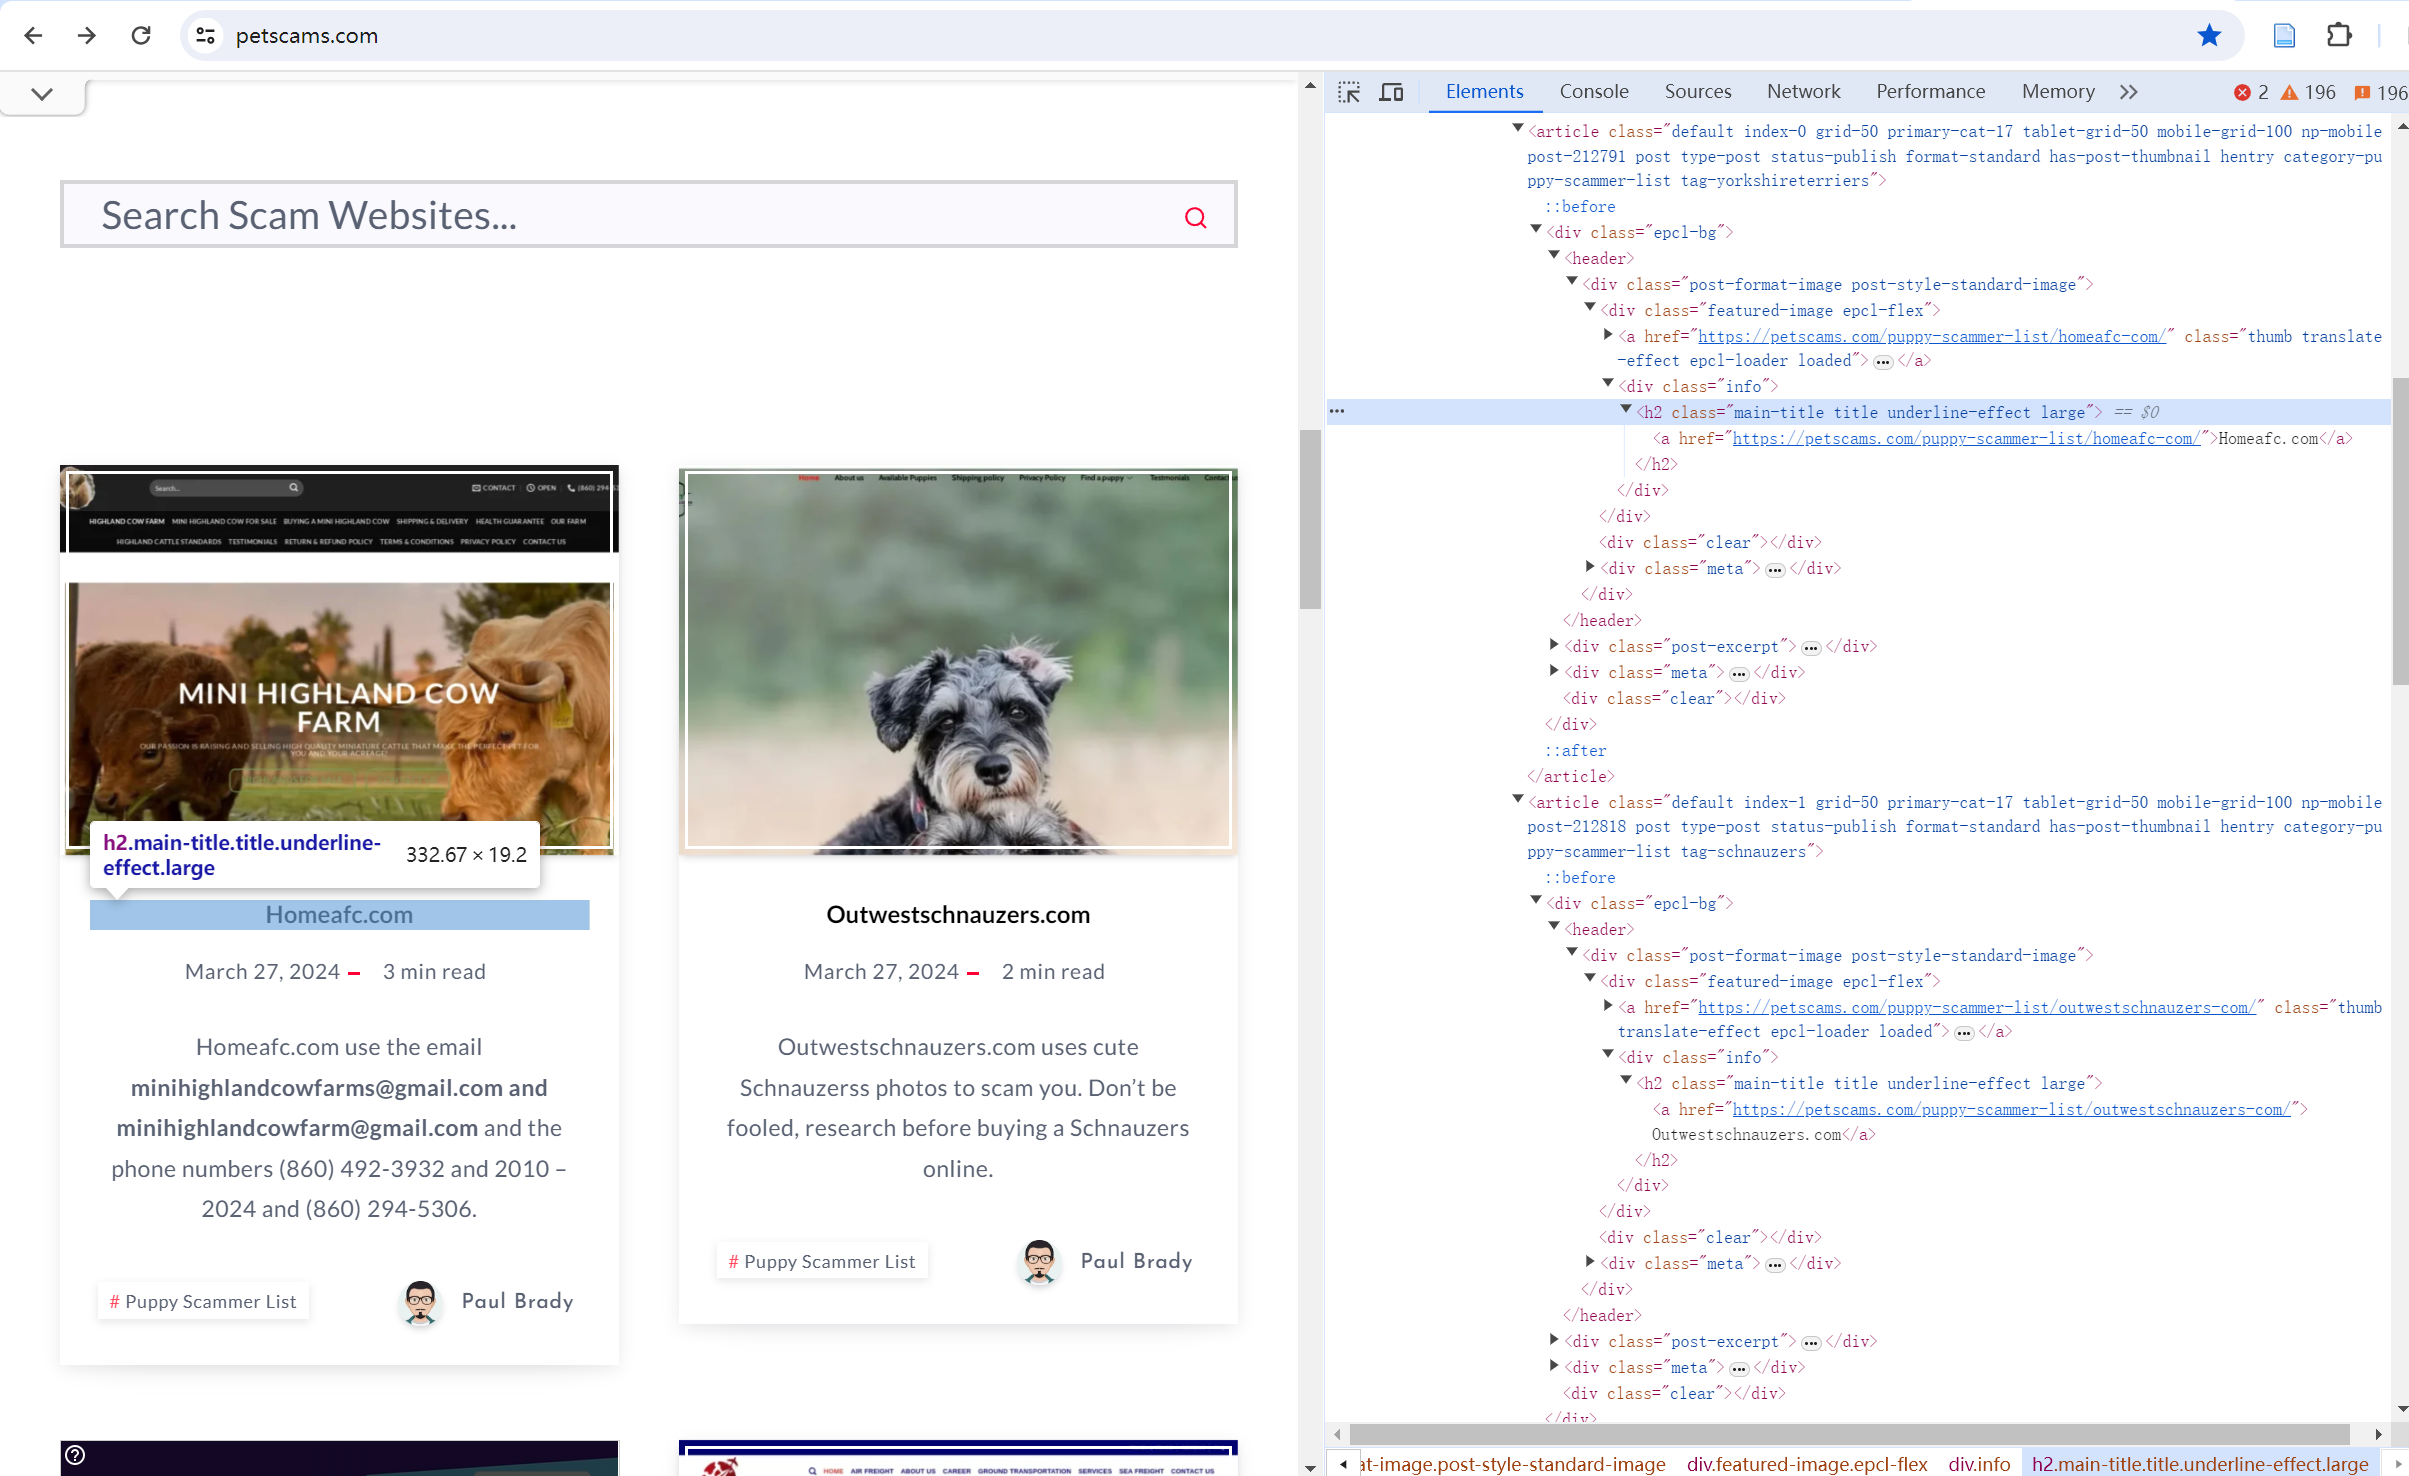
\includegraphics[width=0.8\linewidth,height=0.285\textheight]{pic/figure1.png}
\caption{Petscans.com in the developer mode}
\label{fig:pic1}
\end{figure}

Furthermore, as shown in Figure \ref{fig:pic2} and Figure \ref{fig:pic3}, the page layout across different articles is also remarkably uniform. Each article segments the key points and introductory content, ensuring information is presented clearly. The breakdown of each scam website in the article consists of four main parts - identity, review credibility, legality, and recommended next steps - for in-depth description and analysis. This thoughtful design considerably assists victims and researchers, in quickly and fully understanding the workings of pet scams.
\begin{figure}[H]
    \centering
    \begin{minipage}{0.45\textwidth}
        
\includegraphics[width=\linewidth]{pic/figure2.png}
        \caption{Homeafc.com}
        \label{fig:pic2}
    \end{minipage}
    \hfill
    \begin{minipage}{0.45\textwidth}
        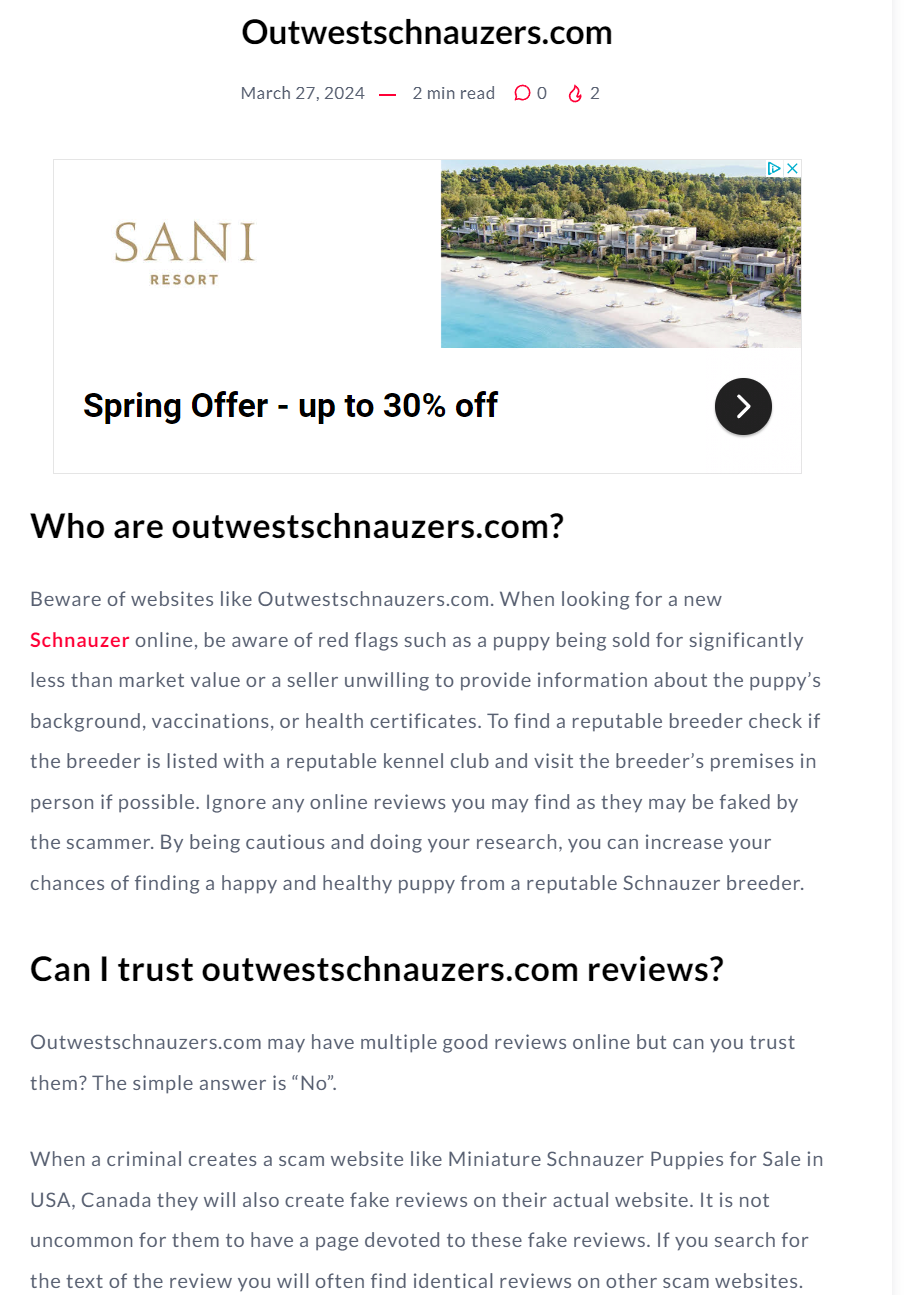
\includegraphics[width=\linewidth]{pic/figure3.png}
        \caption{Outwestschnauzers.com}
        \label{fig:pic3}
    \end{minipage}
\end{figure}


It is indicated that the function of ‘robots.txt’ is to tell search engines which URLs in the site are allowed for crawler access \cite{noauthor_robotstxt_nodate}. By visiting \url{https://petscams.com/robots.txt}, you can understand the scope of web crawling permissions set by the developers, and the text data returned in the page is as follows:
\vspace{10pt}
\noindent\hrule  
\begin{Verbatim}[fontsize=\small]
# START YOAST BLOCK
# ---------------------------
User-agent: *
Disallow:
Sitemap: https://petscams.com/sitemap_index.xml
# ---------------------------
# END YOAST BLOCK
\end{Verbatim}
\hrule  
\vspace{10pt}


It can be seen that the configuration of the file is highly open. The rules specified by \href{https://www.petscams.com}{Petscams.com} permit all search engine crawlers to access all the content on the website, providing a solid foundation for the implementation of web scraping technologies.
\\

\section{Web Scraping}
Compared to traditional manual data collection, web scraping can automatically retrieve unstructured data from a large amount of text such as HTML, then convert it into a structured format and store it locally \cite{khder_web_2021}. As Zhao stated \cite{zhao_web_2017}, the web scraping process mainly includes two parts: acquiring web resources and extracting specific information from the received data. The former refers to accessing the target webpage via the HTTP protocol, while the latter is to parse and extract the necessary data through automated scripts, and then save it in a specific format for further analysis. In this section, we will focus on discussing the most commonly used technology libraries when performing these two stages.
\\

In the first stage of web scraping, communication with the web server needs to be conducted through the HTTP, which is a request-response protocol that supports most web pages \cite{chandra_python_2015}. The Requests library in Python simplifies interaction with the target URL, providing efficient and reliable methods. As one of the most popular HTTP libraries, it supports the use of various HTTP methods, including GET, POST, PUT, and DELETE. Moreover, it also includes advanced features such as handling error and exception, authentication, redirects, sessions and SSL verification \cite{noauthor_requests_nodate}. These features meet all the requirements of the initial steps, ensuring the simplification of obtaining and processing server responses, including headers, session cookies, and status codes.
\\

For the second stage, various tech libraries can be utilised to parse and extract web data. Currently, BeautifulSoup, Selenium, and Scrapy are widely used because of their powerful capabilities. These tools focus on interactions with websites, as well as the extraction and parsing of data, each one demonstrating its own performance and advantages.
\\

BeautifulSoup is a Python library designed for parsing HTML and XML documents. It offers a simple and user-friendly syntax, enabling users to swiftly locate the necessary elements in the parsing tree using selectors like tag names, id names, etc \cite{chandra_python_2015}. For small or medium-sized crawling tasks on static web pages, BeautifulSoup can often be paired with the Requests library to form a lightweight crawling solution. It's important to note that this technology library primarily focuses on parsing work and does not involve constructing concurrent requests \cite{fariha_beautifulsoup_2023}.
\\

Similarly, Selenium does not support concurrent requests, which limits its efficiency in asynchronously executing multi-site scraping tasks to a certain extent. However, as a browser automation tool, Selenium supports multiple programming languages including Python, Java, and C\#, demonstrating unique capabilities in automating web browser operations \cite{fariha_beautifulsoup_2023}. Due to the unique support for JavaScript dynamically loaded pages \cite{fariha_beautifulsoup_2023}, it specialises in simulating human user actions, such as scrolling through pages, filling out forms, and clicking buttons. Additionally, unlike tools that need to be combined with the Requests library to send HTTP requests, scripts written by Selenium can run independently, using its built-in browser control functions to directly access and operate web pages. As the automated form filling will be introduced in project development, Selenium will become an indispensable tool library.
\\

Scrapy is a web crawler framework written in Python, which includes a complete set of web scraping solutions, including request handling mechanisms, data extraction, and database storage \cite{noauthor_intro_nodate}. Utilising the Twisted asynchronous network framework, Scrapy supports efficient concurrent request handling, making it particularly suitable for large-scale data crawling tasks and complex web data collection projects \cite{noauthor_intro_nodate}. Apart from being less self-sufficient in handling JavaScript than Selenium, and new users may encounter a certain learning curve, Scrapy better integrates the key functions of both Requests and BeautifulSoup. Thus, it can complete tasks independently in most scenarios without relying on external libraries.
\\

However, the demand of this project is relatively simple, there is no need to handle a large number of concurrent requests or complex data crawling. Therefore, I finally chose Requests, BeautifulSoup and Selenium as tools for the crawler development, since our main focus is to prioritise the smooth execution of the overall system process. While this approach may not be as comprehensive as Scrapy, it offers sufficient flexibility and convenience to meet project requirements. If necessary, it has also kept a door open for incorporating more efficient and complex crawling technologies in the future.


\section{Recognition and Processing of Text Data}
Throughout the construction and execution of the project system, various types of text data will be encountered, such as form content, email content, and time records. To manage these data effectively, this section introduces various methods for implementing information retrieval, guided by the heuristic search algorithm concept. These methods can be used separately or in combination, to ensure that the system identifies and processes text data accurately and efficiently.
\\

Heuristic search is a goal-oriented searching method. While it doesn't always guarantee the optimal solution, it usually provides high-quality solutions \cite{a_chapter_2001}. The heuristic search algorithm, also known as the A* algorithm, merges the benefits of keyword search and clustering. When dealing with NP problems that have incomplete solving conditions, the following evaluation function is established \cite{zhao_information_2014}:
\\

f(n)=g(n)+h(n)
\\

Here, f(n) represents the total estimated cost of node n, g(n) represents the actual path cost from the beginning state to node n, and h(n) stands for the heuristic estimated cost from node n to the goal. These values can help reflect the distance between the node and the goal, guiding the optimal path with each search step. This algorithm improves search efficiency by avoiding the exploration of invalid paths, thus improving the accuracy of vital information retrieval while ensuring the response speed. Therefore, the essence of heuristic search is to use limited information to achieve the search goal at the lowest cost. After acquiring substantial data through web scraping, this logic can also facilitate the fast batch retrieval of relevant information. Based on the characteristics or patterns of the data items, you can predefine the keyword groups, key data types, and different pattern matches. This allows scripts to execute ``semi-structured" searches, effectively recognising and filtering vast amounts of text \cite{manning_introduction_2009}.
\\

Furthermore, the use of Regex and the FuzzyWuzzy library also demonstrates the application of heuristic search. As Uzum's report \cite{uzun_comparison_2018}, Regex is a sequence of characters that define a search pattern. With the introduction of the ``re" module in Python, a pattern is predefined to extract data. However, this study also found that data extracted using Regex is only 43.5\% accurate compared to the expected data. Therefore, this project will consider using only simple Regex rules to remove unnecessary text information. 
\\

FuzzyWuzzy is a Python library used for string matching. Unlike Regex, once this library is utilised, a relevance score ranging from 0-100 need to be set \cite{majumder_fuzzywuzzy_2021}. The higher the score, the more closely the query word should match the target string. This can also be viewed as the retrieval constraints defined in retrieval heuristics \cite{yang_secure_2021}. By using fuzzy string matching, this heuristic method allows for a wider range of possibilities for a target string with uncertain content, thereby preventing over-matching a single query word.


\section{GPT Models}
In response to the demand for generating a large number of emails, the conventional approach involves using predefined text templates to generate email content. However, for a more advanced automated response system, I decided to integrate the GPT model.
\\

GPT, short for Generative Pre-Trained Transformer, has been extensively pre-trained on natural language data. It can predict and generate subsequent content after receiving text, images, or sound through the transformer \cite{3blue1brown_but_2024}. Since the release of the first \texttt{GPT-1} version in June 2018, \href{https://openai.com/}{OpenAI} has developed numerous models with various functions \cite{noauthor_openai_nodate}. For instance, the GPT series focuses on understanding and generating natural language or code; DALL·E specialises in image generation and editing; Whisper, a voice recognition model, and Jukebox is a music generation model. And these models are still being continuously updated and optimised.
\\

The core requirement of this project is to effectively understand and generate natural language text. In this case, the newly released \texttt{GPT-3.5-turbo-0125} and \texttt{GPT-4-0125-preview} models both meet this requirement well. The processing capabilities of these two models have reached up to 60,000 tokens (approximately 45,000 English words) and 300,000 tokens (approximately 225,000 English words) per minute, respectively. The latter can also reduce the ``laziness" of the model not completing tasks \cite{noauthor_openai_nodate}. This demonstrates that by integrating the API key into the system, adjusting both the necessary prompts and other parameters according to the code template provided by \href{https://openai.com/}{OpenAI} \cite{noauthor_openai_nodate}, AI can automatically generate email content in batches using human language logic. Which will result in an efficient response speed and a natural interaction experience.




\chapter{Project Execution}
\section{Automatic Receipt of Inbound Emails}
Due to the large amount of email correspondence generated when the system induces fraudsters, the demand for the domain mail server has become a primary issue. In this project, two domains called “liveonline.ninja” and “malabaka.social” were registered on \href{https://www.name.com}{Name.com}, which were used for the system's testing and experimental stages in turn. \href{https://www.mailgun.com}{Mailgun.com}, as a scalable email sending platform, is a significant tool for executing this project. Under the guidance of the official documentation \cite{noauthor_domain_nodate}, two domains were added in Mailgun and configured the DNS records to track the key information of all email correspondence under the domain.
\\

As shown in Figure \ref{fig:pic4}, the Logs page of Mailgun allows users to view and track all email content and their statuses under the specified domain within the past five days of communications. However, these log records are automatically deleted after five days. To ensure the 31-days experiment can proceed smoothly, a script named \texttt{email\_crawl.py} was created for automated retrieval and long-term storage of inbound emails. First, configure the Mailgun API key and the required domain name in the system. Then, use the \texttt{request.get()} method to batch transfer emails based on a customised time range and event status. Each email should be named according to its unique receiving time, represented by the Unix timestamp. To ensure readability of the archived email content, the program formats each inbound email by retaining only the title, body, sender, and recipient information. This information is finally stored in a separate JSON file.
\begin{figure}[H]
\centering
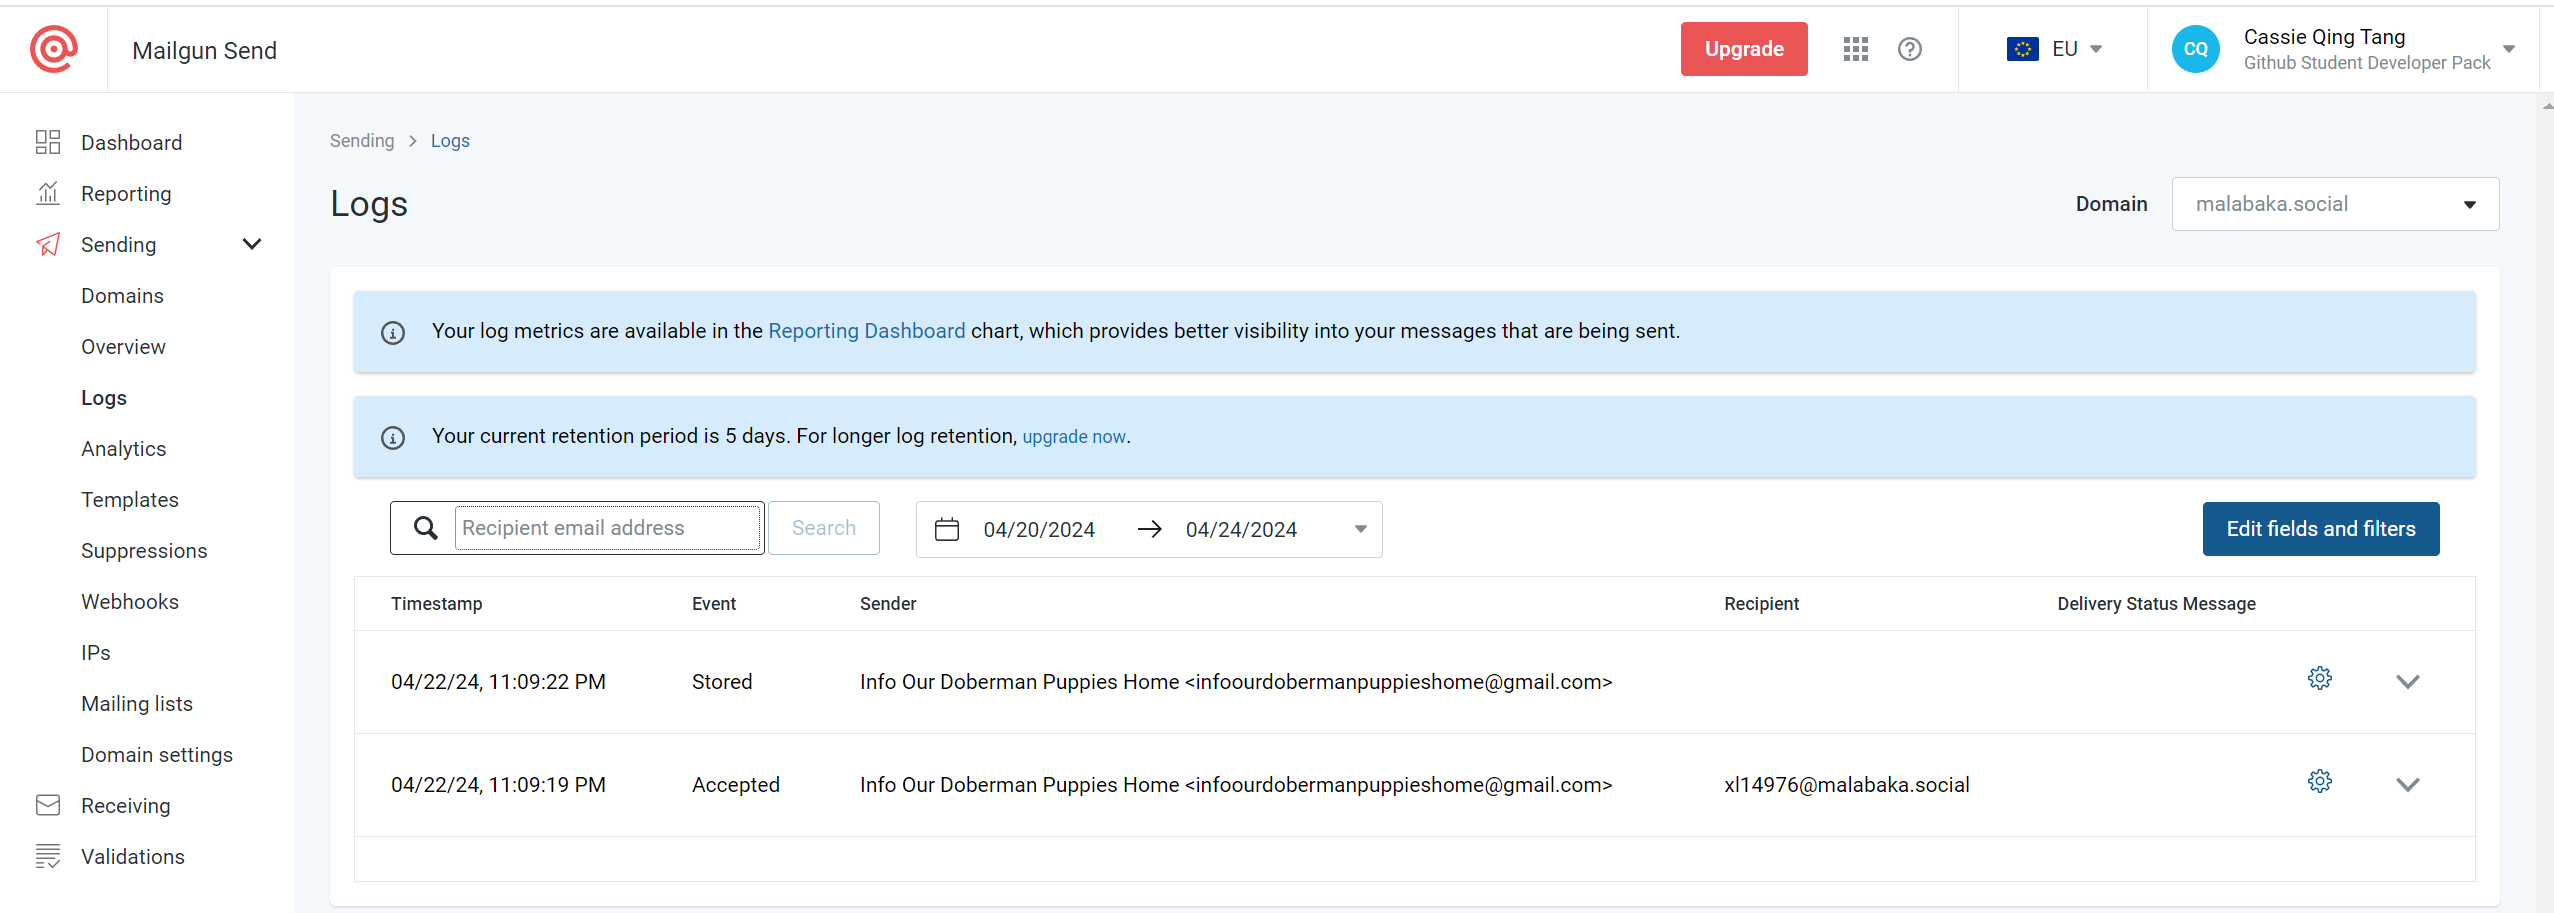
\includegraphics[width=0.95\linewidth,height=0.2\textheight]{pic/figure4.png}
\caption{Mailgun logs page of malabaka.social}
\label{fig:pic4}
\end{figure}


\section{Implementation of Web Scraping}
In this project, web scraping is primarily used to access, collect, and fill in a large amount of data on the form pages of pet scam websites. We have learned before that \href{www.petscams.com}{petscams.com} is a key resource, dedicated to collecting and reporting information on scam websites related to pet sales and transportation. Given that pet transportation scams are often only involved in the later stages of scam activities, and these scam websites do not expect consumers to contact them proactively. Therefore, our crawlers will only focus on those fraudulent pet websites involved in sales.

\subsection{Crawling and Filtering List of Target Websites}
The scraping process begins with \texttt{petscam\_crawl.py}, which targets fake pet sales websites on \url{https://petscams.com/category/puppy-scammer-list/}. It fetches HTML pages using the requests library and parses them with BeautifulSoup using `html.parser'. The script identifies each $<$article$>$ tag, then uses the $<$time$>$ and $<$h2 class=``main-title"$>$ tags within to filter articles by publication date and extract scam domain names.  Each extracted domain is automatically prefixed with `https://' to ensure they are directly accessible.
\\

While randomly visiting some of the URLs reported in recent months, it was found that some of them have already expired or been suspended. This issue is more prevalent with scam domain names revealed earlier. As a result, the code includes checks for the return status code of the link and potential message prompts such as ``Account Suspended" and ``Maintenance mode is on". On the other hand, the administrators of \href{www.petscams.com}{Petscams.com} occasionally re-post the same websites, which can lead to duplicate links saved in the JSON list. Taking advantage of the characteristic that sets do not allow duplicate elements \cite{sturtz_sets_nodate}, all valid URLs are first stored in a set, then converted into a list format and stored in a JSON file. These strategies can effectively prevent the potential waste of time and decrease in accuracy that invalid or duplicate links could cause in the subsequent code execution process.
\\

Next, heuristic search will be used to retrieve the contact form pages that exist in the website list collected in the previous step, which is done by a crawler program called \texttt{contactpage\_crawl.py}. Based on observations of a large number of pet scam sites, scammers usually set up a ``Contact Us" page, guide people to leave their contact information, and thus get in touch with the victims separately. Through Chrome's developer mode, I summarised the three common structures they often use when developing this page, and wrote the code according to them.
\\

Some scam websites place the contact form directly on the main page instead of setting up a separate submission page. Since $<$form$>$ element is frequently used to initiate and nest form content \cite{noauthor_how_2024}, the script first checks for the existence of $<$form$>$ and common elements within it, like $<$input type = ``email"$>$, on the main page. If these exist, the main page's URL is directly used as the target form page URL and stored in a JSON file. If these elements are not found on the homepage, the script continues to search for links containing specific keywords, such as ``contact-us" or ``reach-us". The form links related to these keywords are usually found in the $<$a href$>$ tag. Moreover, some scammers choose to put the form URL contained in the $<$a href$>$ tag in the $<$li$>$ tag instead of $<$form$>$. Thus, the code also includes keyword retrieval for this potential structure.

\subsection{Automated Form-Filling}
After identifying the URL of a scam website's contact page, the system simulates a typical scam process. This is done by a script called \texttt{formfill\_crawl.py}. It uses the Selenium library to render websites in real-time, capturing and dynamically filling form fields generated by JavaScript. Before coding, I analysed multiple pet scam websites that were recently exposed by Petscams.com to identify common patterns in form development. Typically, these forms require basic information such as name, phone number, email address, home address, pet name, and message. However, the illogical nature of these code can only be revealed in developer mode. For instance, some DOM tree structures are overly complex, causing form data to be buried within irrelevant levels or appearing in peer structures where it shouldn't be. Additionally, it is found that some data types are mismatched. For example, a phone number field that should be labelled as ``tel" or ``number" is incorrectly marked as a ``text" type. Multiple fields are also named with unrelated long strings. All these irregular designs aim to disrupt the detection efficiency of automation tools.
\\

In response to these challenges, I abandoned the traditional data recognition method limited to standardised forms and instead implemented a complex dictionary nesting structure \cite{noauthor_python_2023}. This approach enables the specification of detailed recognition rules for each form field, including element types, required attributes, and other common optional attributes. The library of recognition rules has been progressively refined through extensive examination and analysis of fraudulent forms. Meanwhile, the script utilises the FuzzyWuzzy library for fuzzy matching, with the matching threshold set at 90, thereby improving the accuracy of recognition. And the maximum search recursion depth is set to 2, which is sufficient for handling complex multi-level form structures. To enhance efficiency, caching and multi-threading technologies have been introduced, allowing simultaneous processing of different form elements, thereby optimising the utilisation of computing resources elegantly.
\\

In the process of auto-filling forms, it is crucial to maintain the reasonableness and randomness of data to prevent potential issues, such as bothering unrelated individuals. Personal details like names are randomly created by Python library called `names', while email addresses are a combination of random strings and the preset domain name. Even pet names and species are randomly generated. When dealing with logically connected information like phone numbers, addresses, countries, and cities, consistency at the national level is maintained. By using counters and for-loops, the system assigns specific information of either the US or the UK to different forms, thus preventing data confusion within the same form. Furthermore, the message board input uses the \texttt{GPT-3.5} language model and sequentially applies four common strategies to interact with scammers. This approach ensures equal participation opportunities for responders with different personalities. For forms with drop-down selections and check-boxes, the script will automatically and randomly choose options after identifying labels such as ``checkbox", ``radio", or ``select".
\\

Next, \texttt{formfill\_crawl.py} uses Selenium to find and click the submit button, and to check if the form has been sent successfully. The program intercepts network requests of XMLHttpRequest through JavaScript code. It captures and analyses request data in real-time, specifically focusing on the status code and response content of POST requests. This helps to determine whether a form submission has been successful or not. If the network data is not enough to confirm that, the system look for other signs like ``Thank you" or ``success" on the web page. In the end, all important data collected during this process, including the name, email address, scam form URLs, and the time of form filling, are recorded to keep our operation stats up to date. By extracting and testing three sets of real scam forms using the ``liveonline.ninja" domain name, the script achieved a success rate between 45\% and 60\%. Although this didn't meet an expected goal, it is adequate to support the subsequent experimental research needs for this project.


\section{Implementation of Email Automation Responses}
In the email automatic response phase, the system adopted four response strategies that were initially implemented in the message board function: Investigator, Newbie, Bargainer, and Impatient Consumer. These strategies were chosen based on a study of numerous online shopper personalities \cite{noauthor_types_nodate} and a thorough analysis of past pet scam cases \cite{whittaker_understanding_2020}. Our goal is to efficiently waste the time of pet scammers. Emails require dealing with more complex text compared to message boards. For this reason, we utilised \texttt{GPT-4-0125-preview}, the latest advanced text generation model, to satisfy the need for high-quality natural language generation.
\\

In order to safeguard response authenticity and privacy, our system uses regular expressions to eliminate confusing greetings from the start of emails. Also, the system has adjusted the key parameters of the generation model: \texttt{temperature} and \texttt{top\_p} to control the predictability and diversity of the output \cite{noauthor_openai_nodate}. For instance, we set higher values (0.6 and 0.7) for newbies and impatient consumers, enhancing reply naturalness. For bargainers and investigators, we use medium (0.5) and lower (0.3) values respectively, aligning with their communication styles. These adjustments within the GPT language model template \cite{sanders_how_2023} enable us to customise email reply strategies. Take the following code of the function investigator as an example:
\vspace{10pt}
\noindent\hrule 
\lstset{
  basicstyle=\small\ttfamily,
  breaklines=true, 
  showstringspaces=false,
  tabsize=2,                  
  columns=fullflexible, 
}

\begin{lstlisting}[language=Python]
def investigator(prompt):
    prompt = "Reply without any signature :" + prompt
    completion = openai.ChatCompletion.create(
        model="gpt-4-0125-preview",
        messages=[
            {"role": "system",
            "content": "Act as an inquisitive investigator, seeking detailed evidence to confirm the pet sale's validity. Deny being a robot or causing trouble if questioned. Persist in the discussion, avoiding repeat questions and maintaining a logical flow with relevant follow-ups or new queries. If receiving attachments, don't open them and respond that you cannot open them. Maintain privacy and do not use any form of greeting or address such as `Dear [name]' or `Hi [name]'. But you should also make all your reply seem a little more humane."},
            {"role": "user", "content": prompt}
        ],
        temperature=0.3,
        top_p=0.3
    )
    res = completion.choices[0].message.content
    res = re.sub(r"\[.*?\]", "", res)
    return res.strip()
\end{lstlisting}
\hrule  
\vspace{10pt}

The \texttt{corn.py} script is primarily used for centralised replies to batch emails. It parses emails collected by \texttt{email\_crawl.py}, generates appropriate reply text, and then uses the Mailgun module to send the email. To maintain a consistent and credible conversation, this script identifies the proper response strategy by searching the record from the previous script execution. This approach can avoid suspicion caused by sudden strategy changes. Each generated email uses formatting techniques, by simulating the ongoing communication with ``Re:" as the prefix, then adding the signature and username at the end to enhance the authenticity of the response.
\begin{figure}[H]
\centering
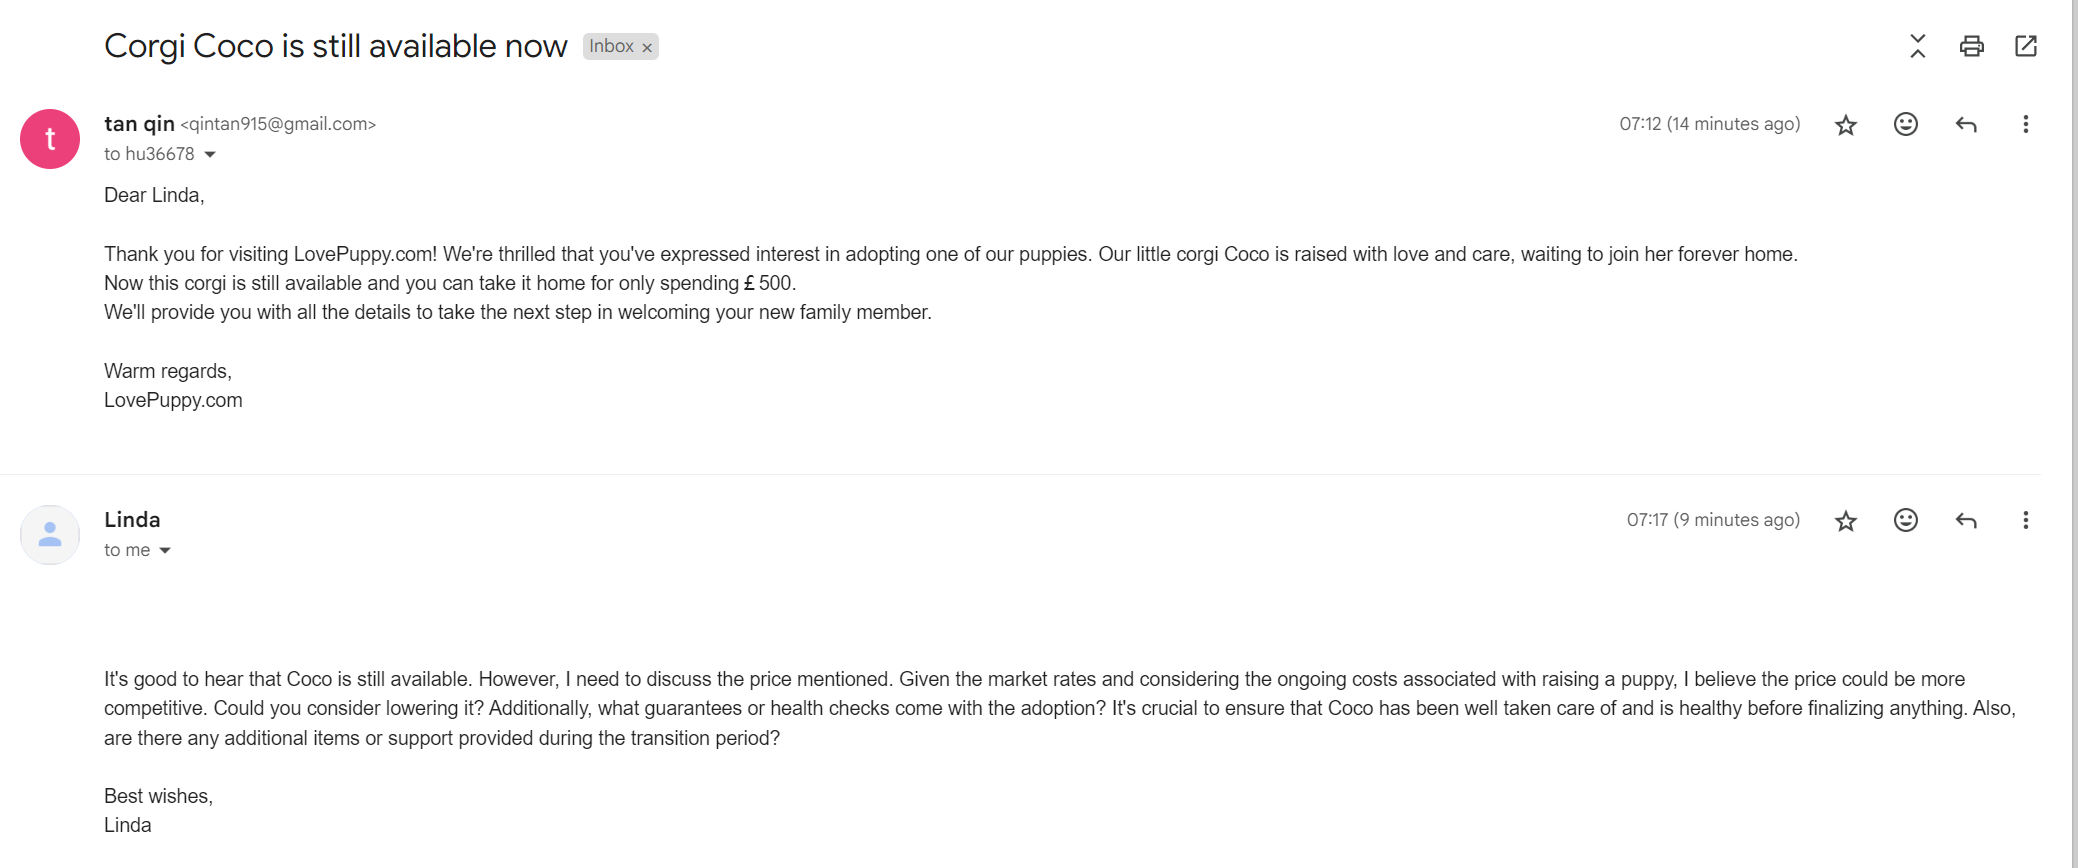
\includegraphics[width=\linewidth, height=0.25\textheight]{pic/figure5.png}
\caption{Email Communication for testing}
\label{fig:pic5}
\end{figure}

As shown in Figure \ref{fig:pic5}, the system acts as a ``bargainer" in response to a test scam email delivered to the system domain via Gmail. Figure \ref{fig:pic6} provides detailed metadata of this email, validating the system's proficiency in handling nuanced communication tasks. It has revealed that the content matching and email format meet the test benchmark, effectively demonstrating the practicality of the script in real email exchanges. In order to prevent system overload and potential crashes, the script also sets a maximum limit on the number of emails and content tokens, thereby effectively managing the load. Simultaneously, it employs an exception-catching mechanism to avoid issues caused by errors.
\begin{figure}[H]
\centering
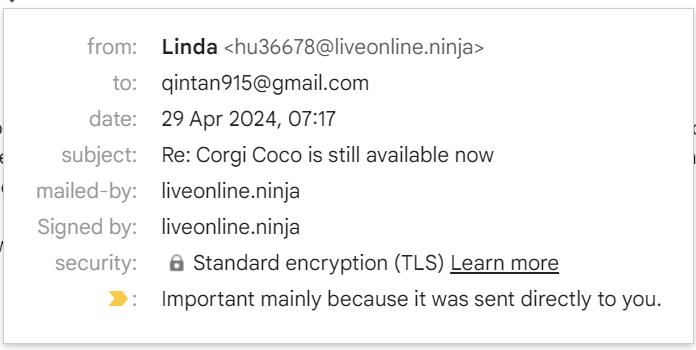
\includegraphics[width=0.4\linewidth]{pic/figure6.png}
\caption{Metadata of this response email}
\label{fig:pic6}
\end{figure}

\section{Construction and Operation of the System}
The system was built on an open-source, expandable scam-baiting mail server \cite{an19352_an19352scambaiter_back_2023}, which eliminates the need to construct a basic architecture from scratch. The simplified development process involved integrating own crawlers, customising the reply procedure for pet scammers and configuring API keys along with data storage directories. Consequently, this section mainly focuses on how these pre-written programs are well organised into a complete system designed to disrupt pet scams.
\\

Despite comprehensive testing of all programs before the experiment's start, real-time error monitoring was vital to ensure an uninterrupted experiment. Instead of merging the five key scripts or enhancing their calling, they were managed and run separately within the project. However, there is an inherent link between these scripts, each producing data stored in JSON format in the system, ready for others to access. After eliminating two irrelevant crawlers and several email reply templates from the original email server, Figure \ref{fig:pic7} and Figure \ref{fig:pic8} clearly show the architecture and operation flow of the system during the two stages of web interaction and email interaction respectively.
\begin{figure}[H]
\centering
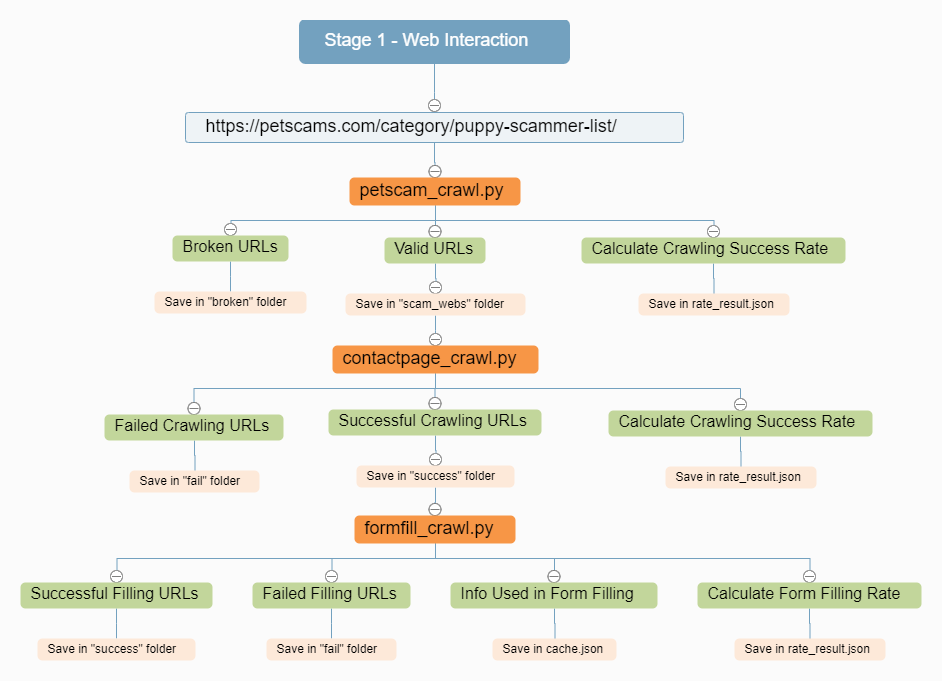
\includegraphics[width=0.8\linewidth]{pic/figure7.png}
\caption{Stage 1 - Web Interaction}
\label{fig:pic7}
\end{figure}

\begin{figure}[H]
\centering
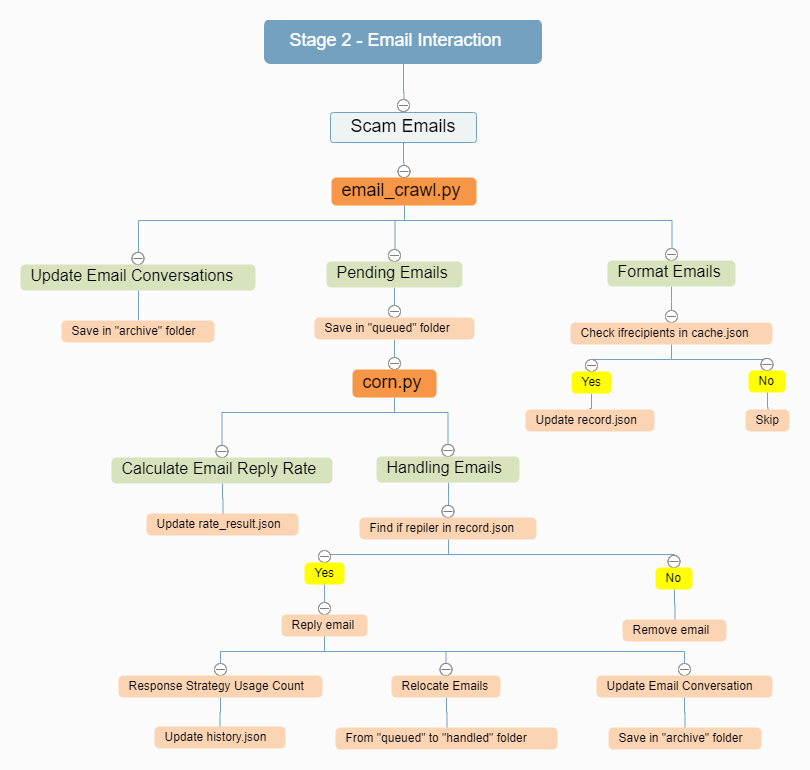
\includegraphics[width=0.8\linewidth]{pic/figure8.png}
\caption{Stage 2 - Email Interaction}
\label{fig:pic8}
\end{figure}

Figure \ref{fig:pic7} illustrates the system's first stage workflow, specifically, the interaction process with pet scam pages. This flowchart clearly outlines each step, from initial crawling to data processing. Each step involves storing the URL crawling results, and all the data is saved in JSON file format. The system also calculates the success rate of each script based on the number of successfully captured links and attempts, which is vital for monitoring and optimising the crawler's performance. The entire process's progression relies on accurately reading and processing valid data.
\\

Figure \ref{fig:pic8} shows the second stage of the email handling process, which involves processing emails from the Mailgun domain server. During this stage, all incoming scam emails are archived for future review and sorted into the processing queue. In addition, each email's recipient information is compared with the data in the \texttt{cache.json} file from the first stage. If the data matches, it means that the email originated from the form-filling activity in the first stage. Details from matched emails, such as the email address of scammers and the timestamp of the email, are automatically stored in the \texttt{record.json} file. This file also contains the reply strategy for deciding whether to reply to the email, which is executed through the corn.py script. After each reply to a new scammer, the \texttt{history.json} file is updated to track the usage frequency of various reply strategies.
\\

After finishing the coding and thorough testing of the project, I scheduled the experiment to start on March 15th (Friday) and end on April 15th. Regular visits to \href{www.petscams.com}{petscams.com} showed that the website updates approximately every 2-3 days, with each update publishing around 15 articles exposing fraudulent pet sales platforms. Given this pattern, and considering the success rate of \texttt{formfill\_crawler.py}, I divided the 31-day experiment into four cycles. Apart from the first Friday of the first week, when it was necessary to interact with pet scam pages exposed within the past 30 days, the following three Fridays required interactions with pages exposed within the past 7 days only. This approach ensured continuous communication with the scammers throughout the experiment and facilitated the collection of diverse data. Also, during the experiment, I needed to respond to new emails daily between 5pm and 7pm. Accounting for the 4-5 hour time difference, this time corresponds to 12pm to 3pm Eastern Time in the United States, a period of high activity for Americans. In the previous text, we have already learned that the United States is not only one of the first countries to expose online pet scams but also the country where these scams occur most frequently. Therefore, sending emails during this time period increases the likelihood of timely responses, even from scammers located in Europe. More detailed information about the experimental process is shown in Figure \ref{fig:pic9}.
\begin{figure}[H]
\centering
\includegraphics[width=\linewidth]{pic/figure9.png}
\caption{The Process of Experiment}
\label{fig:pic9}
\end{figure}


\chapter{Critical Evaluation}
\label{sec:4}
\section{Script Performance Analysis}
\subsection{Performance of Scam Page Interaction Scripts}
As the experiment progressed, the system automatically logged execution data for each script, including duration and success rate. This data is summarised in Table \ref{tab:table1}, which clearly illustrates the performance of the three scripts responsible for interaction with pet scam pages.
{\small
\begin{table}[ht]
\centering
\renewcommand{\arraystretch}{1.5}
\resizebox{\textwidth}{!}{
\begin{tabular}{@{}|c|c|c|c|c|c|c|@{}}
\toprule
\textbf{Date} & \textbf{Script Name} & \textbf{Duration (s)} & \textbf{Scraped Links} & \textbf{Attempted Links} & \textbf{Success Rate (\%)} & \textbf{Avg Time Per Link (s)} \\
\midrule
Mar 15 & contactpage\_crawl & 386 & 325 & 334 & 97.3\% & 1.16 \\
Mar 22 & contactpage\_crawl & 53 & 42 & 42 & 100.0\% & 1.26 \\
Mar 29 & contactpage\_crawl & 51 & 44 & 45 & 97.8\% & 1.13 \\
Apr 5 & contactpage\_crawl & 65 & 43 & 44 & 97.7\% & 1.48 \\ \hline
Mar 15 & petscam\_crawl & 702 & 334 & 334 & 100.0\% & 2.10 \\
Mar 22 & petscam\_crawl & 97 & 42 & 42 & 100.0\% & 2.31 \\
Mar 29 & petscam\_crawl & 104 & 45 & 45 & 100.0\% & 2.31 \\
Apr 5 & petscam\_crawl & 110 & 44 & 44 & 100.0\% & 2.50 \\ \hline
Mar 15 & formfill\_crawl & 9254 & 146 & 325 & 44.9\% & 28.47 \\
Mar 22 & formfill\_crawl & 1587 & 19 & 44 & 69.0\% & 37.79 \\
Mar 29 & formfill\_crawl & 1373 & 27 & 44 & 61.4\% & 31.20 \\
Apr 5 & formfill\_crawl & 1445 & 22 & 43 & 51.2\% & 33.60 \\
\bottomrule
\end{tabular}
}
\caption{Summary of script performance metrics}
\label{tab:table1}
\end{table}
} 

The table also contains the average processing time of the script on links, which is determined by dividing the duration by the number of attempted links. This directly shows the efficiency of each script. In particular, \texttt{petscam\_crawl.py} maintained a 100\% success rate throughout the experiment. This was due to the regular structure of the target website, \href{www.petscams.com}{Petscams.com}, and our script being tailored to this structure. Similarly, \texttt{contactpage\_crawl.py} also achieved a high success rate of over 97\%, with efficiency twice that of \texttt{petscam\_crawl}. The occasional link capture failures were mainly due to non-English interface websites, absence of key positioning words, or the lack of the contact page on some scam websites.
\\

Compared to the first two, \texttt{formfill\_crawl.py} performs less effectively, with a success rate of only 44.9\%-69\%. However, this is relatively similar to the 45\%-65\% result obtained by the same script during the test phase. Regarding the reasons for the form auto-filling failures, my collection and analysis of the failed pages during the experiment led to the following conclusions:
\begin{itemize}
  \item Unable to pass the robot verification on several websites, which is a problem that most auto-fill scripts still cannot solve.
  \item Some websites may not accept mobile numbers containing special symbols, such as the plus sign (+). However, the mobile phone information that the system can automatically fill in always starts with the US country code +1 or the UK country code +44.
  \item The script has certain technical limitations when dealing with forms that contain multiple similar required fields. For instance, as the form shown in Figure \ref{fig:pic10}, even though both `First' and `Last' fields under `Name' are mandatory, the script struggles to fill in another field after recognising and filling one with a matching name attribute.
  \item Unpredictable special text requirements can also lead to auto-filling failures. For example, the unfilled text boxes in Figure \ref{fig:pic11} are due to the script not being pre-set to recognise such special long sentence information.
\end{itemize}
\begin{figure}[H]
    \centering
    \begin{minipage}{0.45\textwidth}
        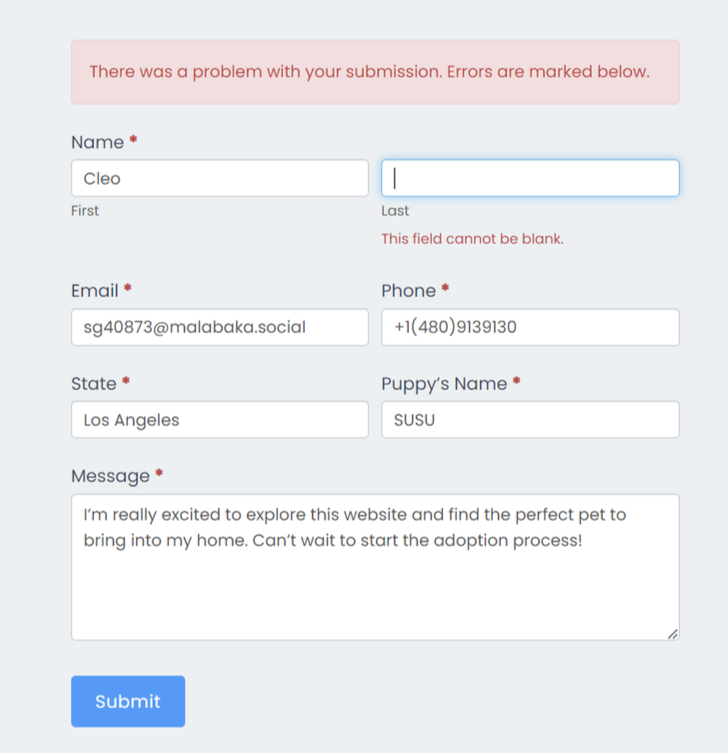
\includegraphics[width=\linewidth]{pic/figure10.png}
        \caption{Incomplete `Name' Field Error}
        \label{fig:pic10}
    \end{minipage}
    \hfill 
    \begin{minipage}{0.45\textwidth}
        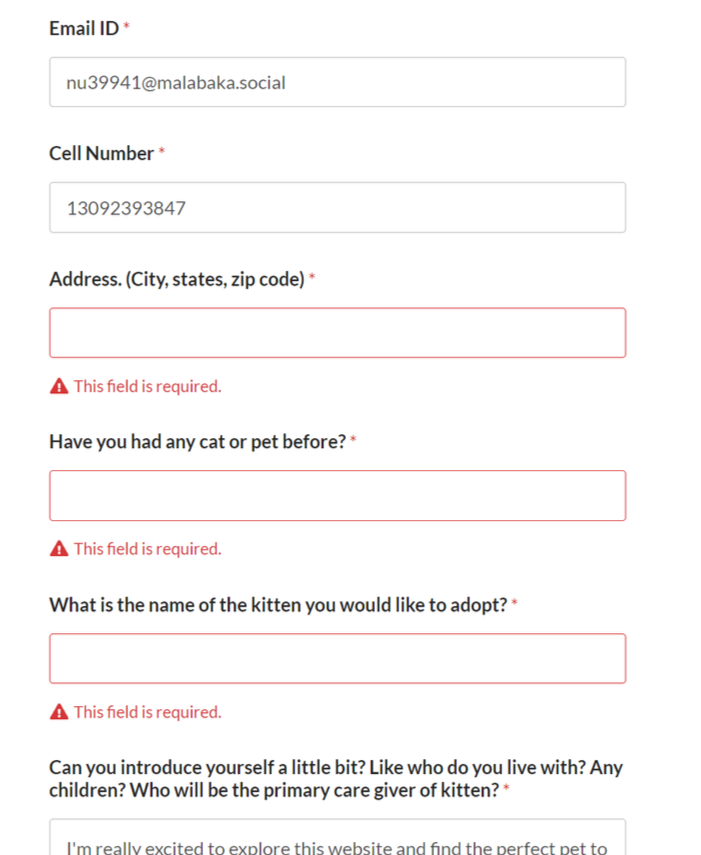
\includegraphics[width=\linewidth, height=0.3\textheight]{pic/figure11.png}
        \caption{Unrecognised Text Error in Form}
        \label{fig:pic11}
    \end{minipage}
\end{figure}

The problem mentioned above was identified on the first day of the experiment. At that time, I considered potential solutions, such as enhancing the heuristic algorithm to recognise and fill more elements or even replacing it with a deep learning algorithm for graphical forms. However, I was cautious about introducing unpredictable changes that could potentially cause more issues, so I did not modify the relevant code. Additionally, Table \ref{tab:table1} indicates that the average processing time for automatic form filling is quite long. Particularly on March 22\textsuperscript{nd}, it took an average of 37.79 seconds to process a link, even though it had the highest success rate on that day. In fact, this slower speed can be anticipated, as the complexity of this script code is significantly greater than the first two. Factors such as the recognition of a large, nested dictionary structure, multi-level recursive searches, and the time required for submission checks all contribute to its efficiency. Moreover, the impact of the network environment each time the script is executed should also be considered. Therefore, such fluctuations in processing time are reasonable.
\\

Even though the success rate and efficiency of \texttt{formfill\_crawler} are not very ideal, each respondent has tried a sufficient number of submissions as shown in Table \ref{tab:table2} during form filling. In this way, they are more likely to get equal participation opportunities in subsequent email replies. Overall, the same script exhibits minimal error in the running data across different experimental cycles. This demonstrates a consistent correlation and stability between the success rate and processing time, indicating that the script is approaching maturity.
\begin{table}[ht]
\centering
\begin{tabular}{@{}lc@{}}
\toprule
\textbf{AI Responder} & \textbf{Submission Count} \\
\midrule
Investigator & 67 \\
Newbie & 57 \\
Bargainer & 59 \\
Impatient Consumer & 54 \\
\bottomrule
\end{tabular}
\caption{Number of form submissions by each AI responder}
\label{tab:table2}
\end{table}

\subsection{Status of Email Sending and Receiving}
The system keeps detailed records of the daily email sending and receiving activities during the experiment. These records include the date, daily counts of received and successfully sent emails, as well as the success rate of email responding. Theses are used to plot a line chart as seen in Figure \ref{fig:pic12}, which shows the trend of the email response rate over time.
\begin{figure}[H]
\centering
\includegraphics[width=\linewidth]{pic/figure12.png}
\caption{Daily Email Delivery and Response Performance from March 16 to April 15}
\label{fig:pic12}
\end{figure}

The line chart shows that on the first day of email replies, the success rate was only 73.9\%, with 12 emails failing to receive replies. This issue occurred because the original experimental procedure only allowed \texttt{formfill\_crawl} to store data related to successfully submitted forms in \texttt{cache.json}. Generally, this mechanism should be effective. However, on March 15\textsuperscript{th}, during a high volume of table submissions, the script inaccurately assessed the submission results. This happened because some websites did not return the expected 200 status code. Therefore, despite the website indicating that the form submission was successful, the system backend wrongly recorded the failure message ``Form submission failed or confirmation not found". As a result, even though the scammer had successfully received these form data and sent scam emails, the system could not find the corresponding recipient record in \texttt{cache.json}, resulting in the automatic reply not being triggered.
\\

In order to address this misjudgement and prevent the experiment from ending prematurely, after discussing with my supervisor, I decided to make some adjustments before completing the forms for the second cycle. The specific operation requires modifying just two lines of code, enabling \texttt{cache.json} to store key information from both successful and unsuccessful attempts. This then allows for a complete system re-test. This change ensures the system retains sufficient information to respond to scammers' email in the event of a misjudgement, without affecting the smooth progression of the experiment.
\\

This adjustment has immediately improved the stability of sending and receiving emails. As demonstrated in the subsequent weeks, the daily volume of sent and received emails remained essentially constant, only occasionally failing due to invalid scam domains. Moreover, as shown in Figure \ref{fig:pic12}, although the volume of emails sent and received throughout the experiment showed a gradual declining trend, there were still 5 emails sent and received on the last day, successfully meeting the experiment's expectations.

\section{The Scammer's Response to the System}
\subsection{Analysis of Scammer Response Rates}
\label{sec:4.2.1}
Generally, online scammers often rush to implement scams, which makes them respond quickly after receiving form submissions. Under the system setting, the number of respondents and scammers is a one-to-one match. Therefore, by counting the number of new reply strategies at the end of each cycle and dividing it by the total number of forms successfully submitted that week, the response rate of scammers to the system can be essentially estimated. The detailed results are shown in Table \ref{tab:table3}.
{\small
\begin{table}[ht]
\centering
\resizebox{\textwidth}{!}{
\begin{tabular}{@{}ccccccc@{}}
\toprule
\textbf{Experiment Period} & \textbf{New Scammers} & \textbf{Successfully Submitted Forms} & \textbf{Scammers' Response Rate (\%)} \\
\midrule
Week 1 & 34 & 146 & 23.29 \\
Week 2 & 9 & 29 & 31.03 \\
Week 3 & 10 & 27 & 37.04 \\
Week 4 & 11 & 22 & 50.00 \\
\midrule
Total/Average & 64 & 224 & 28.57 \\
\bottomrule
\end{tabular}
}
\caption{Email Response Rate of Pet Scammers to the System}
\label{tab:table3}
\end{table}
} 

Before the experiment, I reviewed the research on pet scam websites conducted by Matthew and Benjamin \cite{price_resource_2020}, which found that some scammers might be the masterminds behind numerous separate scam websites. This suggests that we may encounter scammers managing a large number of pet scam websites during the experiment. And if they realise that different websites have received forms that filled with the same domain name within a certain period, they may become more vigilant and stop sending scam emails. Based on this conjecture, I predicted that the response rate of scammers to the system will gradually decrease during the experiment.
\\

However, Table \ref{tab:table3} shows results that are entirely opposite to the forecast. Specifically, the scammers' response rate to the system has been increasing over time. During the experimental process, the forms filled in the first week covered some pet scam websites that had been exposed earlier. These scammers may not have been as active during the experiment, which could explain why the first week's response rate was only 23.29\%. However, even if the forms filled out are all from pet scam websites exposed in the past 7 days, the trend of the response rate in the subsequent three weeks did not match the prediction. Therefore, the change in the scammers' response rate during the experiment appears to be random and without clear patterns. It's worth noting that this does not contradict Matthew and Benjamin's research results. It merely indicates that there is no obvious connection between these scammers. Alternatively, they might be so greedy or careless that they did not carefully check the domain information filled in forms.
\\

In order to understand the overall response of the scammers to the system during the experiment, the last row of Table \ref{tab:table3} shows the total number of scammers involved in email interactions and the total number of successfully submitted forms. It then divides the two to get the average response rate. This value reached 28.57\%, which means that nearly three out of every ten scammers who received the form actively sent emails to the system. Although this response rate is not high, it can generally produce good results under a large base of form filling. As in this experiment, the system successfully established the email communication with 64 real pet scammers within a month and interfered with their pet scam implementations to different extents.

\subsection{Analysis of Scam Tactics Used in Email Conversations}
\label{sec:4.2.2}
After the experiment, numerous email conversation records were stored in the “archive” folder. In this section, I categorised these email records based on the rounds in conversation and analysed the commonalities and characteristics of the scam content. In this study, the successful receipt and sending of an email are defined as a round of conversation, or called a set of messages. By counting the number of rounds between the system and each scammer, I have summarised these data and conducted a detailed statistical analysis, including calculating the minimum, maximum, average, and median. Based on these analyses, the average is finally decided to be used as the main classification criteria, since it reflects the central tendency of all messages. According to this criteria, each email conversation is divided into three periods: early stage (from the minimum to half of the average), middle stage (from half of the average to 1.5 times the average), and late stage (exceeding 1.5 times the average up to the maximum). Specific classification results are shown in Table \ref{tab:table4}, which includes the number of scammers who persisted to different periods and the distribution of corresponding response strategies.
\begin{table}[H]
\centering
\begin{tabular}{@{}lccccc@{}} 
\toprule
Period & Count & Investigator & Newbie & Bargainer & Impatient Consumer \\ 
\midrule
Early (1-3) & 33 & 12 & 3 & 10 & 8 \\
Midterm (4-11) & 17 & 0 & 7 & 6 & 4 \\
Late (12-48) & 14 & 1 & 7 & 0 & 6 \\
Total  & 64 & 13 & 17 & 16 & 18 \\
\bottomrule
\end{tabular}
\caption{Scammer Interaction and Strategy Usage by Period}
\label{tab:table4}
\end{table}

From this table, it can be seen that half of the scammers abandoned the dialogue with the system within the first three days. After examining the specific email content, I found that the length of the conversation and the reply strategy are closely related. For instance, the ``Investigator" and ``Bargainer" strategies are almost only effective in the early and midterm stages of dialogue. These two strategies respectively played the professional roles of interviewer and bargainer, excelling at identifying information gaps in scammer emails, and posing various questions about pet health certificates, information safety, and costs. In particular, the Investigator, whose responses often included numbered questions, may contain many professional inquiries that scammers did not anticipate, putting them under pressure. Therefore, only one person persisted in targeting the investigator for fraud, and their conversation ended on the 35th round.
\\

In contrast, the performances of the other two strategies are more stable. Their diversity in language and naturalness in emotion made the topics of communication more diversified, not limited to sensitive topics such as the cost and authenticity of online pet sales. Since online pet purchases are relatively new for Newbies, these individuals typically raised just one or two basic questions in an email, which left many new questions to continue the dialogue. Meanwhile, scammers believed that such people were easy to deceive, so they were more willing to invest their time. A similar situation also occurred with the Impatient Consumer. Although this personality was more likely to lose patience in communication, their anxiety about pet orders might also make scammers mistakenly believe that as long as these anxious questions were answered, a transaction could be promoted. As shown in Table \ref{tab:table4}, scammers are more willing to invest their time in these seemingly easy-to-manipulate potential victims.
\\

While the system recorded email conversations from 64 different scammers, a detailed analysis of their email content revealed that they frequently employ similar scam tactics across various respondents. For instance, in just the first email in the early stage, it was found that 49 scammers used very similar template emails or automated responses.
\begin{figure}[H]
\centering
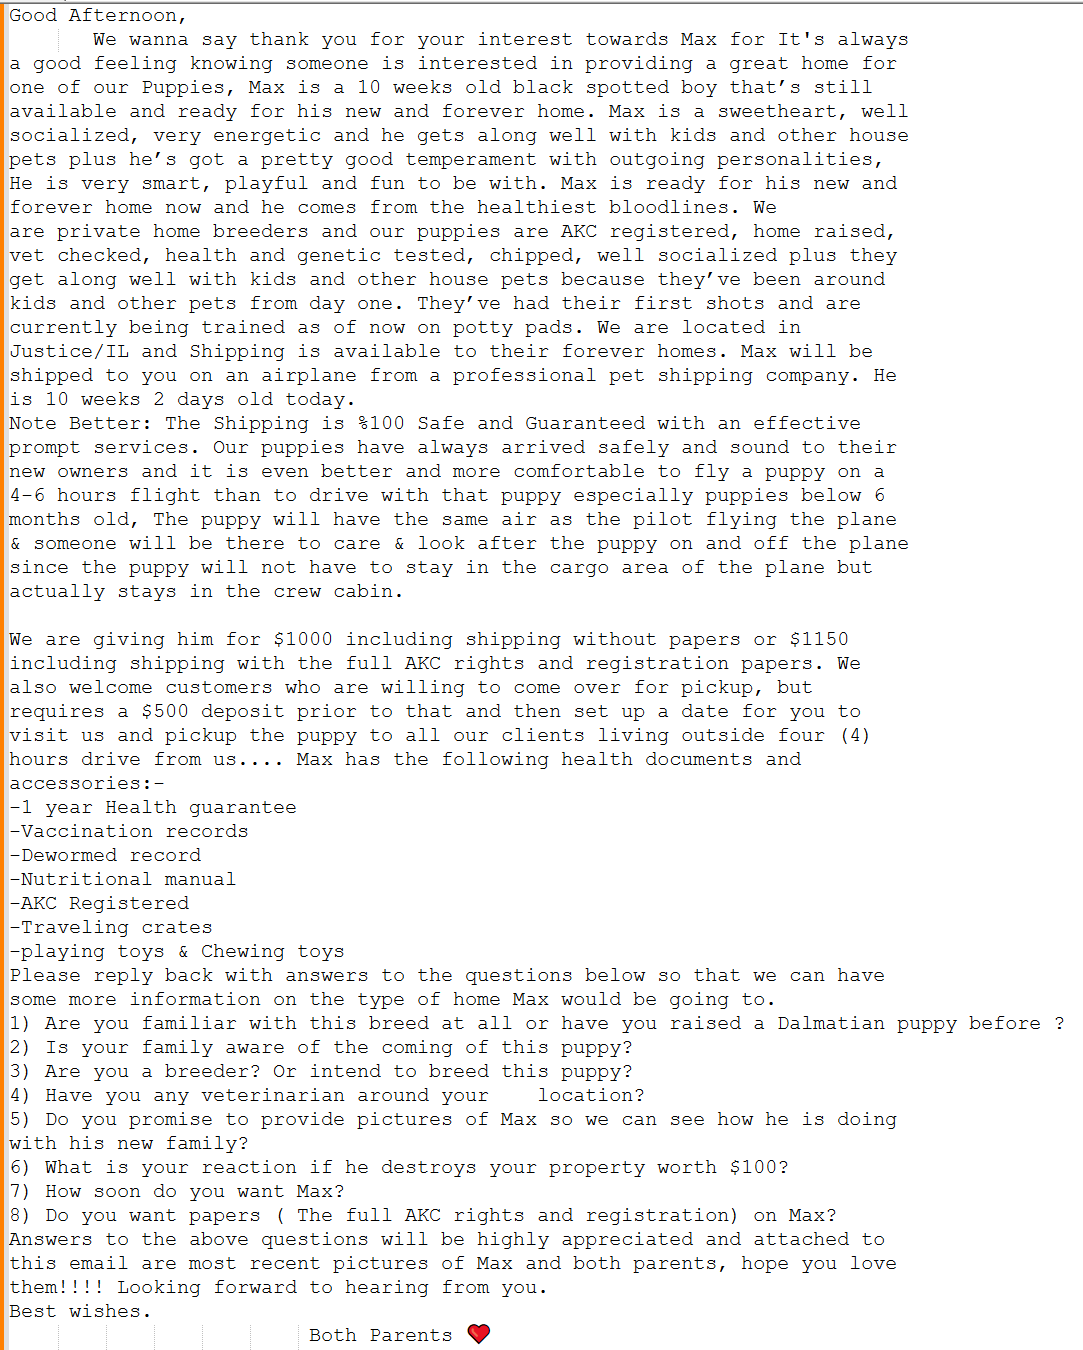
\includegraphics[width=0.7\linewidth]{pic/figure13.png}
\caption{First Scam Email from Dalmatianhomepty@gmail.com}
\label{fig:pic13}
\end{figure}
As shown in Figure \ref{fig:pic13}, this type of email typically begins with a detailed description of the pet's current status, asserts that the pet has been registered with the AKC (American Kennel Club), discusses fees, and finally requests the personal information of potential victims. Interestingly, even though the script randomly filled in the name as Max on the scam form, and there is no puppy named Max on this website, the scammer kept mentioning Max's health status as if this puppy truly existed. According to statistics, at least 36 scammers have used this template in their initial email. Additionally, another 13 fraudsters used a different template, typically sending the content of the system-submitted form as an automatic receipt email. The extremely quick response time of these emails, such as the email in Figure \ref{fig:pic14} which was sent to the domain name server of ``malabaka.social" just 69 seconds after the form was submitted, suggests they are automated replies.
\begin{figure}[H]
\centering
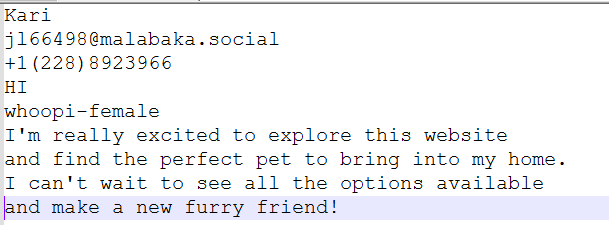
\includegraphics[width=0.35\linewidth]{pic/figure14.png}
\caption{An Auto-Reply Email from info@purrfectdevonrex.com}
\label{fig:pic14}
\end{figure}
The template response was not only used in the first email but also used in other messages from multiple scammers. Other template responses can be triggered if the AI respondent asks questions that were preset by the scammers. For example, during a conversation between Newbie and a scammer, since the system's settings do not allow clicking on any links sent by the scammer, Newbie asked about the content in the link and sent almost the same email three times, each time triggering the same reply.
\\

In most email exchanges, these templated responses primarily used in the early and early-middle stages. Even some manually replied emails were typically responded to in a more patient and polite manner. However, towards the end of the midterm, many scammers began rushing the transaction. By the later period, their tone became increasingly anxious and emotional, attempting to persuade potential victims to complete the payment through various guarantees.
\begin{figure}[H]
\centering
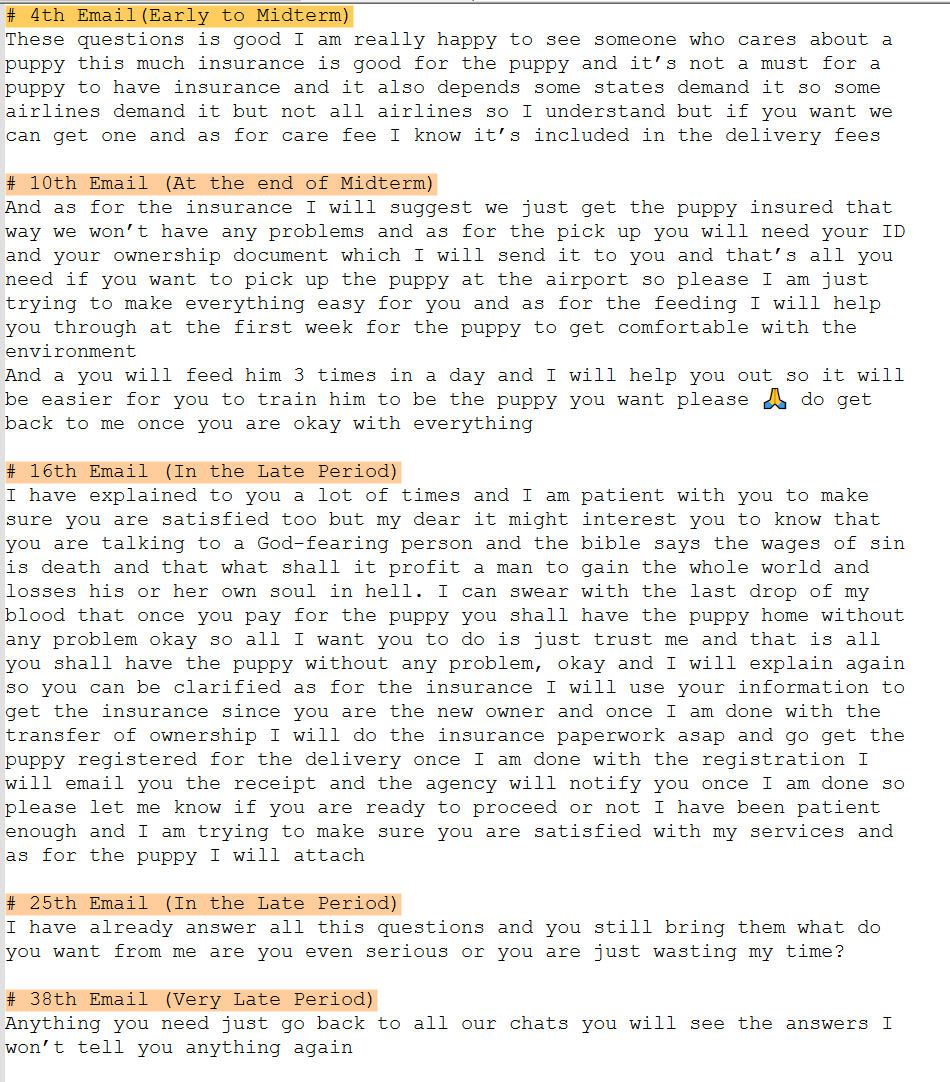
\includegraphics[width=0.6\linewidth]{pic/figure15.png}
\caption{Emails from Andylabradorretrieverhome@gmail.com at Different Periods}
\label{fig:pic15}
\end{figure}
Figure \ref{fig:pic15} shows several messages sent from a scammer at various periods, significantly reflecting the trend described earlier. Especially in the 16th email, the scammer even used the Bible to prove his sincerity. Similar rhetoric has also been recorded in previous research by Whittaker and Button \cite{whittaker_understanding_2020}. By the 25th email, the scammer had already realised that he had been fooled, but he didn't give up on this scam until after the 38th email. In fact, this pattern is the linguistic change that most pet scammers who have had long-term interactions with the system generally experience. After realising that their time has been wasted, these scammers usually show obvious anger, some threaten to block or report emails, and some directly cut off replies. However, regardless of the outcome, these scammers have already had 14 to 28 days of time and energy wasted by the system, effectively interfering with their pet scam plans. Within 9 days after the end of the experiment, the system still received four different emails asking whether there was still interest in buying pets, showing the persistent enthusiasm of pet scammers.

\subsection{Analysis of Repetitive Issues in Email Responses and Their Causes}
\label{sec:4.2.3}
Similar to the behaviours of some scam emails, the system occasionally repeated similar or previously asked questions. However, it was not due to the use of an automatic reply template. In fact, I emphasised the importance of avoiding repetitive questions while designing prompts for generating email text to prevent this phenomenon. However, this preventive measure did not produce the desired result.
\\

In the first week of the experiment, I found that some scammers stated in their responses that the asked question was already answered, suggesting a review of previous emails. This led me to understand the real issue, which was that the system did not reference the relevant email history when generating replies, but only considered the content of the emails received that day. In fact, when building this auto-reply function, I did consider the necessity of reading email history. However, I was concerned that if the system had to deal with all the history related to a specific email, the amount of text processed each time might exceed the limit of 300,000 tokens (about 225,000 English words) that the \texttt{GPT-4-0125-preview} model can handle per minute. Therefore, I chose a solution that uses only a single email as input, and thought that the record of the previous email usually kept at the end of the email would provide the necessary context for generating the reply.
\\

However, looking back at the experimental data in Figure \ref{fig:pic12}, it is evident that the number of emails requiring daily processing did not exceed 50. And the performance of \texttt{corn.py} only supports automatic replies to 5-6 emails per minute, far from approaching the limit of 300,000 tokens per minute(TPM). This ultimately suggests that my excessive concerns have led to irrational design choices.

\section{Comparison of Response Strategies}
After collecting statistical data on the duration and the rounds of email conversation between each reply strategy and scammer, I used various statistical methods including calculating averages, median sorting, and extreme value analysis. The relevant key data results are shown in Table \ref{tab:table5}. This section aims to determine the most effective reply strategy through the comparative analysis of these data.
{\small
\begin{table}[ht]
\centering
\renewcommand{\arraystretch}{1.6}
\resizebox{\textwidth}{!}{
\begin{tabular}{@{}|c|c|c|c|c|c|c|@{}}
\toprule
\textbf{Strategy Name} & \textbf{Average Rounds} & \textbf{Median Rounds} & \textbf{Average Duration (h)} & \textbf{Median Duration (h)} & \textbf{Max Rounds} & \textbf{Max Duration (h)} \\ 
\midrule
Investigator & 3.92 & 1 & 48.02 & 0 & 35 & 552.52 \\ \hline
Newbie & 11.35 & 9 & 184.15 & 191.62 & 48 & 561.87\\ \hline
Bargainer & 3.44 & 3 & 65.56 & 55.62 & 9 & 216.85\\ \hline
Impatient Consumer & 10.78 & 6 & 188.07 & 119.82 & 44 & 669.08\\ 
\bottomrule
\end{tabular}
}
\caption{Comparison of response strategies across various metrics}
\label{tab:table5}
\end{table}
} 

From the table, it can be seen that the median duration of the Investigator is 0 hours. This is because the calculation of duration is based on the timestamp difference between the last email and the first email from the scammer. Combined with the data shown in Table \ref{tab:table4}, we know that most Investigators ended their strategies in the early stage, and usually these conversations had no follow-up after replying to the scammer's first template email or automatic reply, thus not wasting any of the scammer's time.
\\

Comparing the data in Table \ref{tab:table5}, it can be found that Newbie and Impatient Consumer significantly outperform Investigator and Bargainer in all metrics. These higher values indicate that they can communicate with scammers for a longer time, wasting more of the scammer's time, thereby more effectively disrupting scam activities. In addition, the Investigator had 35 email rounds with a scammer that lasted 552.52 hours, indicating that the Investigator strategy may perform exceptionally well when communicating with some particularly professional and patient scammers. Meanwhile, although the Bargainer exceeds the Investigator in both average and median duration, it does not exhibit particularly outstanding performance, making it the most mediocre strategy.
\\

Considering that Newbies and Impatient Consumers perform similarly on key figures, I further applied the U-test to calculate the p-value for the conversation rounds and duration between these two strategies. This helps determine if there's a statistically significant difference between them. Based on the method proposed by Mann and Whitney in 1947 \cite{mann_test_1947}, the U-test involves ranking two independent samples and calculating the sum of ranks, then using these sums to estimate the U-statistic, and finally finding the p-value in the standard normal distribution table through the Z value.
\\

Considering the complexity and potential for error in manually calculating the U-test, I used the \texttt{mannwhitneyu} function \cite{noauthor_scipystatsmannwhitneyu_nodate} integrated in Python to simplify the calculation, which resulted in a p-value of 0.302 for the rounds of conversation and a p-value of 0.397 for the duration. These p-values are higher than the commonly used significance threshold of 0.05, suggesting no statistically significant difference between Newbies and Impatient Consumers regarding the rounds and duration of conversation. Nevertheless, Table \ref{tab:table4} has revealed that Newbie participated more in long-term dialogues, and according to Table 5, Newbie also performed better in terms of the conversation rounds and median conversation duration. Hence, after considering various factors, Newbie is evaluated as the most effective reply strategy. Additionally, I conducted a pairwise p-value comparison of other response strategies, ultimately determining a priority order of effectiveness for the four strategies: Newbie \textgreater{} Impatient Consumer \textgreater{} Bargainer \textgreater{} Investigator. Specific data can be viewed in Table \ref{tab:p_values} of \texttt{Appendix}.


\chapter{Conclusion}
In conclusion, I have successfully built an automatic response system, applying multiple automated scripts to disrupt with online pet scams. This mainly includes building two crawlers that extract HTML text using the \texttt{BeautifulSoup} and \texttt{requests} libraries in Python. The collected pet scam URLs were used as targets for a large amount of contact form filling. Then, the use of the \texttt{Selenium} library helped me identify and automatically fill in form texts, thereby realising an automatic script that can interact with JavaScript dynamic pages. The domain mail server built on \href{www.mailgun.com}{Mailgun} and the well-organised data classification storage helped to achieve the sending and receiving of emails, which was inseparable from the support of four response strategies generated by the GPT language model.
\\

In the experiment, the two scripts used to crawl the basic URLs, \texttt{petscam\_crawl} and \texttt{contactpage\_crawl}, showed a success rate close to 100\%. Similar high-efficiency performance also appeared in the \texttt{email\_crawl} script used for daily email archiving. However, despite multiple improvements to the \texttt{formfill\_crawl} script, the success rate of form submission could only be maintained between 44\% - 70\%, and it has not been able to reach the initial target of over 80\%. This is due to the complex and diverse structure of scam forms, which is difficult to fully predict.
\\

On the first day of the experiment, when running \texttt{corn.py} to respond to scammers' emails, the email response rate was only 73.9\%. After discovering that this problem was due to the misjudgement during form submission, I promptly modified the data storage range in \texttt{cache.json}, successfully raising the subsequent email response success rate to over 93\%. Furthermore, by classifying scam texts by duration and conducting targeted analysis, I found that scammers generally use email templates and automatic replies in their emails. Moreover, as time goes on, the emotional expression of scam email content becomes more and more obvious. In the end, through statistical analysis on the dialogue duration and message quantity of different strategies, including using \texttt{U-test} and other statistical methods, I assessed that the reply strategy named ``Newbie" most effectively disrupted pet scam activities among the four strategies. The evaluation and analysis results of the above scripts are detailed in the \texttt{Chapter} \ref{sec:4} of the paper.
\\

Regarding the actual execution effect of the automatic response system in the experiment, I believe there are still many areas that need to be improved, the first of which is \texttt{formfill\_crawl} with the lowest success rate. Currently, this script uses a complex dictionary nesting structure for form recognition, which is convenient for adding and adjusting at any time. However, to maintain a high text recognition rate, this structure requires the developer to constantly accumulate enough experience to continue updating more scam form elements. In addition, the performance of this recognition method is not ideal as the process from opening to submitting a form requires an average of 32.77 seconds. In the testing phase of the project, I actually thought of some better alternatives.For instance, modify the present heuristic search recognition to deep learning for graphic forms and object detection for form structures. This adjustment will adapt the variable form structure in scam websites, thereby enhancing the accuracy and speed of form recognition. However, due to my insufficient knowledge reserve in machine learning and deep learning, the time cost of relearning is too high. In order to prioritise the successful completion of the project, I gave up optimising this script. However, this is definitely a method worth researching and trying. If I have another chance to retry this project, I will prioritise this method when writing \texttt{formfill\_crawl}. Because I believe that the success of this method will bring more accurate form recognition and better efficiency. Furthermore, the maturity of automated form filling will also bring a better future for this project, since it can be integrated with other systems for classifying fraudulent advertisements or websites, such as the system developed by Ronel for automatically detecting pet scam websites \cite{mehmedov_automated_2021}.
\\

Secondly, in \texttt{Section} \ref{sec:4.2.3}, we have discussed the feasibility and importance of allowing the system to read archives when replying to scam emails. Even after \href{https://openai.com/}{OpenAI} officially reduced the token limit of the \texttt{GPT-4} language model to 30,000 TPM on April 9th \cite{noauthor_openai_nodate}, the plan to let \texttt{corn.py} read the history when replying to emails remains feasible. In this plan, we can set the maximum number of emails and text tokens that can be processed in \texttt{corn.py}, according to the limit of 30,000 TPM and the context window limit of 128,000 tokens. Error handling logic can also be added to the code, so that even if the token limit is exceeded during the request, the program won't crash immediately, but will maintain the smooth progress of the email reply by waiting and trying again.
\\

In \texttt{Section} \ref{sec:4.2.1}, I analysed the changes in the email response rate of the scammers to the system under four experimental cycles, and obtained a response rate that grew over time. This result is completely contrary to my prediction, and it does not conform to the relevant research that Matthew and Benjamin have done \cite{price_resource_2020}. Since scammers generally do not actively contact us if they feel that they will be induced to fraud, I can only temporarily attribute this changing trend to randomness and no obvious rules. But this interesting result is worth further research. If I have the chance, I plan to do more cycles of experiments, collect more data, to determine whether the response rate of the scammers is in line with my initial expectations.
\\

In the end, I am not completely satisfied with the overall architecture of the system. Although the current decentralised architecture successfully supports the independent operation and error checking of scripts in experiments, it is still not mature in terms of structure. Therefore, I plan to integrate these independently running scripts by having them call each other, and completely convert the JSON data stored in the system to database management. This not only facilitates the retrieval and analysis of the captured data but also avoids the system page appearing unorganised.

% \bibliographystyle{ieee}
\bibliography{references}

\appendix

\chapter{Appendix}
\section{Pairwise P-value Comparison of Four Response Strategies}
\label{appendix}

\begin{table}[htbp]
\centering
\begin{tabular}{@{}llcc@{}}
\toprule
Strategy A & Strategy B & P-value (Rounds of Conversation) & P-value (Duration) \\ \midrule
Investigator & Newbies & 0.00072 & 0.0010 \\
Investigator & Bargainer & 0.0056 & 0.0025 \\
Investigator & Impatient Consumer & 0.0167 & 0.0168 \\
Newbies & Investigator & 0.00072 & 0.0010 \\
Newbies & Bargainer & 0.0035 & 0.0221 \\
Newbies & Impatient Consumer & 0.3022 & 0.3972 \\
Bargainer & Investigator & 0.0056 & 0.0025 \\
Bargainer & Newbies & 0.0035 & 0.0221 \\
Bargainer & Impatient Consumer & 0.3288 & 0.4553 \\
Impatient Consumer & Investigator & 0.0167 & 0.0168 \\
Impatient Consumer & Newbies & 0.3022 & 0.3972 \\
Impatient Consumer & Bargainer & 0.3288 & 0.4553 \\
\bottomrule
\end{tabular}
\caption{P-value comparisons for each strategy pair}
\label{tab:p_values}
\end{table}





\end{document}
